\documentclass[8pt,ignorenonframetext,]{beamer}
\setbeamertemplate{caption}[numbered]
\setbeamertemplate{caption label separator}{: }
\setbeamercolor{caption name}{fg=normal text.fg}
% ADD MANU
% \setbeameroption{hide notes}  
% \setbeameroption{show notes}  
\setbeameroption{show notes}   
\setbeamertemplate{note page}[plain]  
%% END ADD MANU
\beamertemplatenavigationsymbolsempty
\usepackage{lmodern}
\usepackage{amssymb,amsmath}
\usepackage{ifxetex,ifluatex}
\usepackage{fixltx2e} % provides \textsubscript
\usepackage{bbm}
\ifnum 0\ifxetex 1\fi\ifluatex 1\fi=0 % if pdftex
  \usepackage[T1]{fontenc}
  \usepackage[utf8]{inputenc}
\else % if luatex or xelatex
  \ifxetex
    \usepackage{mathspec}
  \else
    \usepackage{fontspec}
  \fi
  \defaultfontfeatures{Ligatures=TeX,Scale=MatchLowercase}
\fi
\usecolortheme{dolphin}
% use upquote if available, for straight quotes in verbatim environments
\IfFileExists{upquote.sty}{\usepackage{upquote}}{}
% use microtype if available
\IfFileExists{microtype.sty}{%
\usepackage{microtype}
\UseMicrotypeSet[protrusion]{basicmath} % disable protrusion for tt fonts
}{}
\newif\ifbibliography
\hypersetup{
            pdftitle={R\ldots{} for hydrogeologists(?)},
            pdfauthor={Emanuel Huber},
            colorlinks=true,
            linkcolor=red,
            citecolor=Blue,
            urlcolor=blue,
            breaklinks=true}
\usepackage{color}
\usepackage{fancyvrb}
\newcommand{\VerbBar}{|}
\newcommand{\VERB}{\Verb[commandchars=\\\{\}]}
\DefineVerbatimEnvironment{Highlighting}{Verbatim}{commandchars=\\\{\}}
% Add ',fontsize=\small' for more characters per line
\usepackage{framed}
\definecolor{shadecolor}{RGB}{248,248,248}
\newenvironment{Shaded}{\begin{snugshade}}{\end{snugshade}}
\newcommand{\KeywordTok}[1]{\textcolor[rgb]{0.13,0.29,0.53}{\textbf{{#1}}}}
\newcommand{\DataTypeTok}[1]{\textcolor[rgb]{0.13,0.29,0.53}{{#1}}}
\newcommand{\DecValTok}[1]{\textcolor[rgb]{0.00,0.00,0.81}{{#1}}}
\newcommand{\BaseNTok}[1]{\textcolor[rgb]{0.00,0.00,0.81}{{#1}}}
\newcommand{\FloatTok}[1]{\textcolor[rgb]{0.00,0.00,0.81}{{#1}}}
\newcommand{\ConstantTok}[1]{\textcolor[rgb]{0.00,0.00,0.00}{{#1}}}
\newcommand{\CharTok}[1]{\textcolor[rgb]{0.31,0.60,0.02}{{#1}}}
\newcommand{\SpecialCharTok}[1]{\textcolor[rgb]{0.00,0.00,0.00}{{#1}}}
\newcommand{\StringTok}[1]{\textcolor[rgb]{0.31,0.60,0.02}{{#1}}}
\newcommand{\VerbatimStringTok}[1]{\textcolor[rgb]{0.31,0.60,0.02}{{#1}}}
\newcommand{\SpecialStringTok}[1]{\textcolor[rgb]{0.31,0.60,0.02}{{#1}}}
\newcommand{\ImportTok}[1]{{#1}}
\newcommand{\CommentTok}[1]{\textcolor[rgb]{0.56,0.35,0.01}{\textit{{#1}}}}
\newcommand{\DocumentationTok}[1]{\textcolor[rgb]{0.56,0.35,0.01}{\textbf{\textit{{#1}}}}}
\newcommand{\AnnotationTok}[1]{\textcolor[rgb]{0.56,0.35,0.01}{\textbf{\textit{{#1}}}}}
\newcommand{\CommentVarTok}[1]{\textcolor[rgb]{0.56,0.35,0.01}{\textbf{\textit{{#1}}}}}
\newcommand{\OtherTok}[1]{\textcolor[rgb]{0.56,0.35,0.01}{{#1}}}
\newcommand{\FunctionTok}[1]{\textcolor[rgb]{0.00,0.00,0.00}{{#1}}}
\newcommand{\VariableTok}[1]{\textcolor[rgb]{0.00,0.00,0.00}{{#1}}}
\newcommand{\ControlFlowTok}[1]{\textcolor[rgb]{0.13,0.29,0.53}{\textbf{{#1}}}}
\newcommand{\OperatorTok}[1]{\textcolor[rgb]{0.81,0.36,0.00}{\textbf{{#1}}}}
\newcommand{\BuiltInTok}[1]{{#1}}
\newcommand{\ExtensionTok}[1]{{#1}}
\newcommand{\PreprocessorTok}[1]{\textcolor[rgb]{0.56,0.35,0.01}{\textit{{#1}}}}
\newcommand{\AttributeTok}[1]{\textcolor[rgb]{0.77,0.63,0.00}{{#1}}}
\newcommand{\RegionMarkerTok}[1]{{#1}}
\newcommand{\InformationTok}[1]{\textcolor[rgb]{0.56,0.35,0.01}{\textbf{\textit{{#1}}}}}
\newcommand{\WarningTok}[1]{\textcolor[rgb]{0.56,0.35,0.01}{\textbf{\textit{{#1}}}}}
\newcommand{\AlertTok}[1]{\textcolor[rgb]{0.94,0.16,0.16}{{#1}}}
\newcommand{\ErrorTok}[1]{\textcolor[rgb]{0.64,0.00,0.00}{\textbf{{#1}}}}
\newcommand{\NormalTok}[1]{{#1}}
\usepackage{longtable,booktabs}
\usepackage{caption}
% These lines are needed to make table captions work with longtable:
\makeatletter
\def\fnum@table{\tablename~\thetable}
\makeatother
\usepackage{etoolbox}
\AtBeginEnvironment{table}{\tiny}
\usepackage{graphicx,grffile}
\makeatletter
\def\maxwidth{\ifdim\Gin@nat@width>\linewidth\linewidth\else\Gin@nat@width\fi}
\def\maxheight{\ifdim\Gin@nat@height>\textheight0.8\textheight\else\Gin@nat@height\fi}
\makeatother
% Scale images if necessary, so that they will not overflow the page
% margins by default, and it is still possible to overwrite the defaults
% using explicit options in \includegraphics[width, height, ...]{}
\setkeys{Gin}{width=\maxwidth,height=\maxheight,keepaspectratio}

% Prevent slide breaks in the middle of a paragraph:
\widowpenalties 1 10000
\raggedbottom

\AtBeginPart{
  \let\insertpartnumber\relax
  \let\partname\relax
  \frame{\partpage}
}
\AtBeginSection{
  \ifbibliography
  \else
    \let\insertsectionnumber\relax
    \let\sectionname\relax
    \frame{\sectionpage}
  \fi
}
\AtBeginSubsection{
  \let\insertsubsectionnumber\relax
  \let\subsectionname\relax
  \frame{\subsectionpage}
}

\setlength{\parindent}{0pt}
\setlength{\parskip}{6pt plus 2pt minus 1pt}
\setlength{\emergencystretch}{3em}  % prevent overfull lines
\providecommand{\tightlist}{%
  \setlength{\itemsep}{0pt}\setlength{\parskip}{0pt}}
\setcounter{secnumdepth}{0}
\widowpenalties 1 150

\title{R\ldots{} for hydrogeologists(?)}
\author{Emanuel Huber}
\date{Februar 28, 2018}

%----- ADD MANU
\newcommand{\columnsbegin}{\begin{columns}}
\newcommand{\columnsend}{\end{columns}}
%------------ BOLD MATHCAL > \mathbfcal{} ------------%
\DeclareMathAlphabet\mathbfcal{OMS}{cmsy}{b}{n}

% subitems all same size!
\setbeamertemplate{itemize/enumerate body begin}{\normalsize}
\setbeamertemplate{itemize/enumerate subbody begin}{\normalsize}
\setbeamertemplate{itemize/enumerate subsubbody begin}{\normalsize}

\setbeamertemplate{enumerate item}{\normalsize\insertenumlabel.}
\setbeamertemplate{enumerate subitem}{\normalsize\insertenumlabel.\insertsubenumlabel}
\setbeamertemplate{enumerate subsubitem}{%
\normalsize\insertenumlabel.\insertsubenumlabel.\insertsubsubenumlabel}

%\usepackage[dvipsnames]{xcolor}
\definecolor{Blue}{rgb}{0,0,1<}
%------ END ADD MANU
\begin{document}
\frame{\titlepage}

\begin{frame}

\end{frame}

\begin{frame}{Outline}

\begin{itemize}
\tightlist
\item
  Talk 1:

  \begin{enumerate}
  \def\labelenumi{\arabic{enumi}.}
  \tightlist
  \item
    Overview of R
  \item
    potential use for AUG-group
  \end{enumerate}
\item
  Talk 2: Some important concept on R language
\end{itemize}

\begin{block}{Resources}

\begin{itemize}
\tightlist
\item
  for each task (on \url{https://emanuelhuber.github.io/Rcourse/}

  \begin{itemize}
  \tightlist
  \item
    list of best R-package
  \item
    cheat sheets
  \item
    online book/course/tutorial
  \end{itemize}
\item
  some tutorial on P:/RKurs (including data)
\end{itemize}

\end{block}

\end{frame}

\section{Introduction}\label{introduction}

\begin{frame}{Programming language ranking by the IEEE (2017)}

\href{https://spectrum.ieee.org/computing/software/the-2017-top-programming-languages}{Institute
of Electrical and Electronics Engineers ranking}

\includegraphics[width=1.00000\textwidth]{https://spectrum.ieee.org/image/MjkyNzIzNQ.jpeg}

\end{frame}

\begin{frame}{Why R is so popular}

\begin{itemize}
\tightlist
\item
  free and open-source (no licence)
\item
  runs on Linux, Windows and MacOS.
\item
  large community
\item
  many packages available that are documented (help files + vignette)
\item
  can link C, C++, Fortran code
\item
  excellent tools for data analysis (Google, Airbnb, Facebook,
  Microsoft\ldots{})
\item
  high-quality graphics
\item
  object-oriented programming
\end{itemize}

\end{frame}

\begin{frame}{R Environment: GUI and packages}

\columnsbegin
\column{.5\textwidth} 
\includegraphics{imgPres/packages.png}
\column{.5\textwidth} \textbf{More than 12'000 packages!}
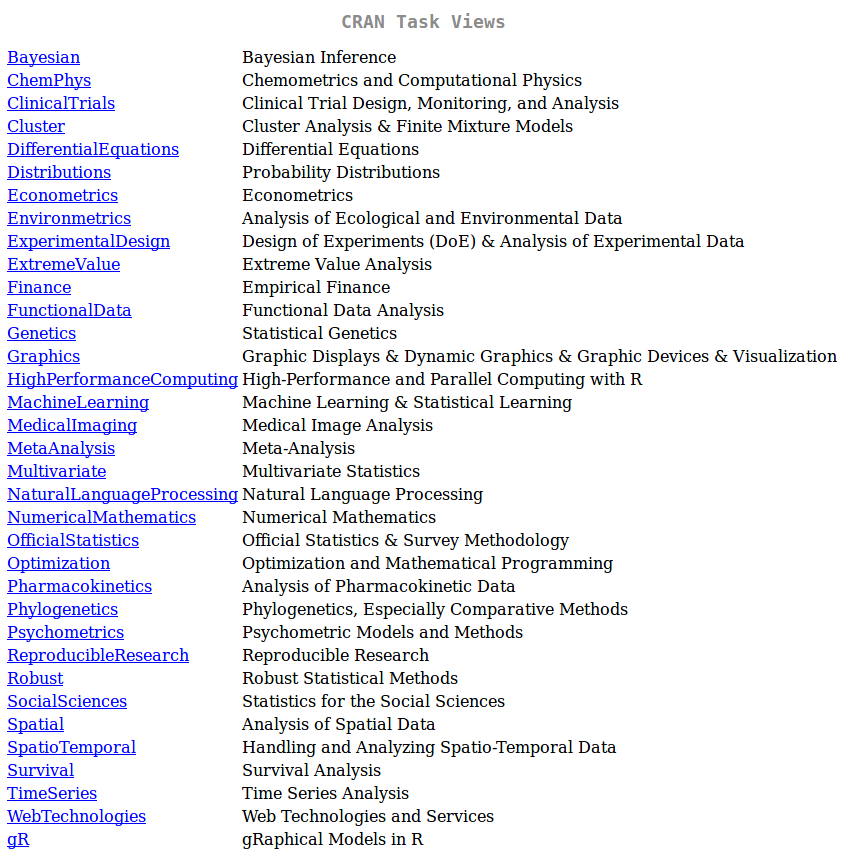
\includegraphics{imgPres/rcran-task-view.png} \columnsend

\end{frame}

\section{Potential use of R for AUG
group}\label{potential-use-of-r-for-aug-group}

\begin{frame}{R strengths}

\columnsbegin

\column{.6\textwidth}

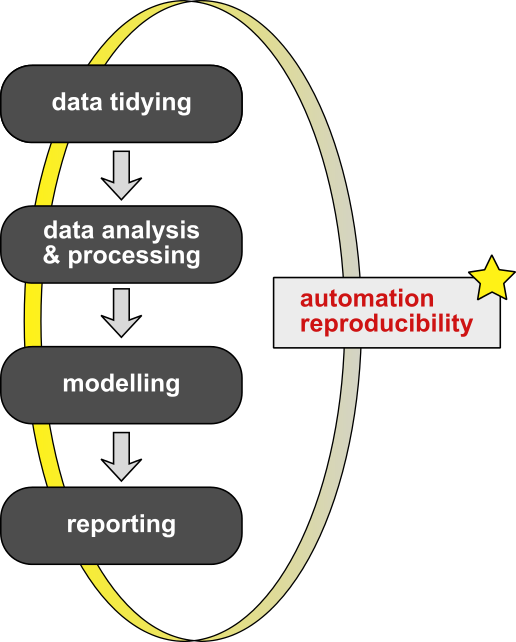
\includegraphics{imgPres/workflow.png}

\column{.4\textwidth}

\begin{itemize}
\tightlist
\item
  all-in-one tool
\item
  no licence
\item
  teaching, research, reporting
\item
  automation and reproducible workflow
\end{itemize}

\columnsend

\end{frame}

\section{Data import/export}\label{data-importexport}

\begin{frame}[fragile]{Resources - data import}

\scriptsize

\begin{longtable}[]{@{}ll@{}}
\toprule
\begin{minipage}[b]{0.25\columnwidth}\raggedright\strut
Function\strut
\end{minipage} & \begin{minipage}[b]{0.69\columnwidth}\raggedright\strut
What It Does\strut
\end{minipage}\tabularnewline
\midrule
\endhead
\begin{minipage}[t]{0.25\columnwidth}\raggedright\strut
\texttt{read.table()}\strut
\end{minipage} & \begin{minipage}[t]{0.69\columnwidth}\raggedright\strut
Reads any tabular data where the columns are separated\strut
\end{minipage}\tabularnewline
\begin{minipage}[t]{0.25\columnwidth}\raggedright\strut
\strut
\end{minipage} & \begin{minipage}[t]{0.69\columnwidth}\raggedright\strut
\texttt{read.table(file\ =\ "filePath",\ sep\ =\ "\textbackslash{}t",\ header\ =\ TRUE)}\strut
\end{minipage}\tabularnewline
\begin{minipage}[t]{0.25\columnwidth}\raggedright\strut
\texttt{read.csv()}\strut
\end{minipage} & \begin{minipage}[t]{0.69\columnwidth}\raggedright\strut
A simplified version of read.table() to read CSV files.\strut
\end{minipage}\tabularnewline
\begin{minipage}[t]{0.25\columnwidth}\raggedright\strut
\strut
\end{minipage} & \begin{minipage}[t]{0.69\columnwidth}\raggedright\strut
\texttt{read.csv(file\ =\ "filePath")}\strut
\end{minipage}\tabularnewline
\begin{minipage}[t]{0.25\columnwidth}\raggedright\strut
\texttt{scan()}\strut
\end{minipage} & \begin{minipage}[t]{0.69\columnwidth}\raggedright\strut
Finer control over the read process when your data isn't tabular.\strut
\end{minipage}\tabularnewline
\begin{minipage}[t]{0.25\columnwidth}\raggedright\strut
\strut
\end{minipage} & \begin{minipage}[t]{0.69\columnwidth}\raggedright\strut
\texttt{scan("filePath",\ skip\ =\ 1,\ nmax\ =\ 100)}\strut
\end{minipage}\tabularnewline
\begin{minipage}[t]{0.25\columnwidth}\raggedright\strut
\texttt{readLines()}\strut
\end{minipage} & \begin{minipage}[t]{0.69\columnwidth}\raggedright\strut
Reads text from a text file one line at a time.\strut
\end{minipage}\tabularnewline
\begin{minipage}[t]{0.25\columnwidth}\raggedright\strut
\strut
\end{minipage} & \begin{minipage}[t]{0.69\columnwidth}\raggedright\strut
\texttt{readLines("filePath")}\strut
\end{minipage}\tabularnewline
\begin{minipage}[t]{0.25\columnwidth}\raggedright\strut
\texttt{read.fwf()}\strut
\end{minipage} & \begin{minipage}[t]{0.69\columnwidth}\raggedright\strut
Read a file with dates in fixed-width format.\strut
\end{minipage}\tabularnewline
\begin{minipage}[t]{0.25\columnwidth}\raggedright\strut
\strut
\end{minipage} & \begin{minipage}[t]{0.69\columnwidth}\raggedright\strut
\texttt{read.fwf("filePath",\ widths\ =\ c(1,\ 2,\ 3)}\strut
\end{minipage}\tabularnewline
\begin{minipage}[t]{0.25\columnwidth}\raggedright\strut
\texttt{readxl::read\_excel()}\strut
\end{minipage} & \begin{minipage}[t]{0.69\columnwidth}\raggedright\strut
To read excel files (xls and xlsx), from
\href{https://cran.r-project.org/web/packages/readxl/index.html}{\texttt{readxl}}
package\strut
\end{minipage}\tabularnewline
\begin{minipage}[t]{0.25\columnwidth}\raggedright\strut
\strut
\end{minipage} & \begin{minipage}[t]{0.69\columnwidth}\raggedright\strut
\texttt{read\_excel("filePath",\ sheet\ =\ "mtcars")}\strut
\end{minipage}\tabularnewline
\bottomrule
\end{longtable}

\end{frame}

\begin{frame}{Import/export}


\includegraphics{imgPres/input.png}

\end{frame}

\section{Data preparation}\label{data-preparation}

\begin{frame}[fragile]{Resources - data cleaning}

\begin{itemize}
\tightlist
\item
  \textbf{Package}

  \begin{itemize}
  \tightlist
  \item
    \href{https://cran.r-project.org/web/packages/dplyr/index.html}{\texttt{dplyr}}
  \end{itemize}
\item
  \textbf{Cheat sheet}

  \begin{itemize}
  \tightlist
  \item
    \href{https://www.rstudio.com/wp-content/uploads/2016/09/RegExCheatsheet.pdf}{regular
    expression cheat sheet}
  \item
    \href{https://github.com/rstudio/cheatsheets/raw/master/data-transformation.pdf}{\texttt{dplyr}:
    data transformation cheat sheet}
  \end{itemize}
\item
  \textbf{Tutorials/book}

  \begin{itemize}
  \tightlist
  \item
    \href{https://cran.r-project.org/doc/contrib/de_Jonge+van_der_Loo-Introduction_to_data_cleaning_with_R.pdf}{Tutorial:
    An introduction to data cleaning with R (53 p.)}
  \item
    \href{https://onepager.togaware.com/DataO.pdf}{Hands-On Data Science
    with R: Data Preparation}
  \item
    \href{https://cran.r-project.org/web/packages/dplyr/index.html}{check
    \texttt{dplyr}-vignettes}
  \item
    \href{https://rstudio-pubs-static.s3.amazonaws.com/74603_76cd14d5983f47408fdf0b323550b846.html}{Tutorial:
    Regular Expressions in R}
  \end{itemize}
\end{itemize}

\end{frame}

\begin{frame}[fragile]{Data cleaning (1)}

\columnsbegin

\column{.6\textwidth}

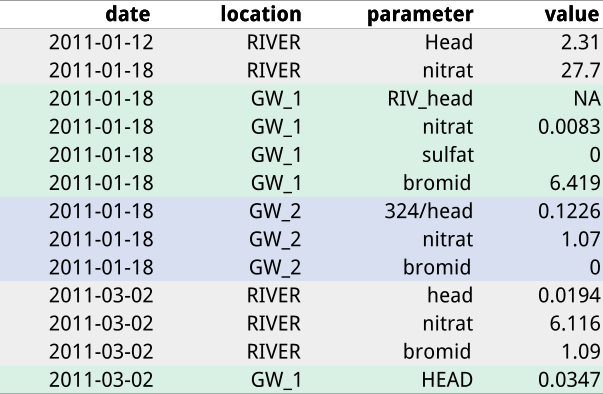
\includegraphics{imgPres/data_tidying_table_messy_bad.png}

\begin{itemize}
\item
  rename variables: \texttt{Head}, \texttt{RIV\_head},
  \texttt{324/head}, \texttt{head}, \texttt{HEAD} -\textgreater{}
  \texttt{head}

\begin{Shaded}
\begin{Highlighting}[]
\NormalTok{pattern <-}\StringTok{ "^RIV_|^[[:digit:]]+/"}
\NormalTok{x$parameter <-}\StringTok{ }\KeywordTok{sub}\NormalTok{(pattern, }\StringTok{""}\NormalTok{, x$parameter)}
\NormalTok{x$parameter <-}\StringTok{ }\KeywordTok{tolower}\NormalTok{(x$parameter)}
\end{Highlighting}
\end{Shaded}
\end{itemize}

\column{.4\textwidth}

\begin{itemize}
\tightlist
\item
  remove rows/columns
\item
  remove duplicates
\item
  transform data
\item
  correct for inconsistencies
\item
  convert data type
\item
  deal with missing values
\end{itemize}

\columnsend

\end{frame}

\begin{frame}{Data cleaning (2)}

\columnsbegin
\column{.7\textwidth}
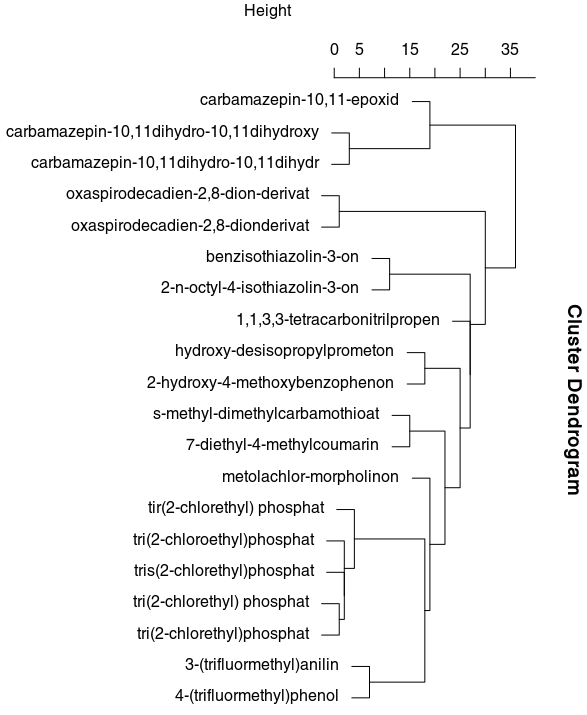
\includegraphics{imgPres/data_cleaning_dendrogram.png}
\column{.3\textwidth} \textbf{detect typo errors} - distance between
strings - dendrogram visualisation - partial string matching \columnsend

\end{frame}

\begin{frame}[fragile]{Resources - data shaping}

\begin{itemize}
\tightlist
\item
  \textbf{Package}

  \begin{itemize}
  \tightlist
  \item
    \href{https://cran.r-project.org/web/packages/tidyr/index.html}{\texttt{tidyr}}
  \end{itemize}
\item
  \textbf{Cheat sheet}

  \begin{itemize}
  \tightlist
  \item
    \href{https://github.com/rstudio/cheatsheets/raw/master/data-import.pdf}{\texttt{tidyr}:
    Tidy Data (see p.~2)}
  \end{itemize}
\item
  \textbf{Tutorials/book}

  \begin{itemize}
  \tightlist
  \item
    Concepts of data tidying are well explained in the chapter
    \href{http://garrettgman.github.io/tidying/}{Data Tidying} from the
    book Data science with R.
  \end{itemize}
\end{itemize}

\end{frame}

\begin{frame}[fragile]{Data shaping 1 (tidy data)}

\columnsbegin
\column{.45\textwidth} ``Messy'' data
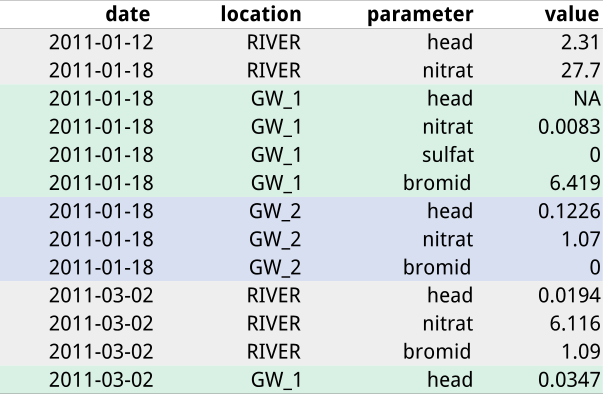
\includegraphics{imgPres/data_tidying_table_messy.png}
\column{.45\textwidth} Tidy data satisfies three rules
(\href{http://garrettgman.github.io/tidying/}{see Data Science with R}):

\begin{itemize}
\tightlist
\item
  Each variable in the data set is placed in its own column
\item
  Each observation is placed in its own row
\item
  Each value is placed in its own cell
\end{itemize}

\columnsend

Tidy data

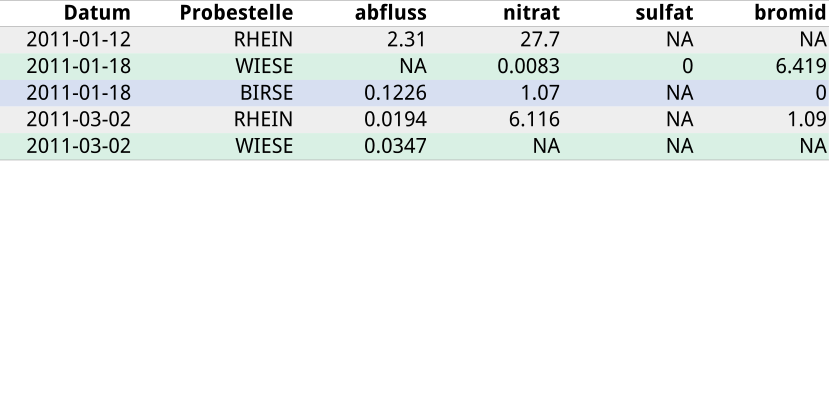
\includegraphics[width=0.70000\textwidth]{imgPres/data_tidying_table_tidy.png}

\begin{Shaded}
\begin{Highlighting}[]
\NormalTok{x_tidy <-}\StringTok{ }\NormalTok{tidyr::}\KeywordTok{spread}\NormalTok{(x, parameter, value)}
\end{Highlighting}
\end{Shaded}

reverse process possible

\end{frame}

\section{Data analysis and
processing}\label{data-analysis-and-processing}

\begin{frame}{Data analysis}

\begin{itemize}
\tightlist
\item
  data analysis

  \begin{itemize}
  \tightlist
  \item
    statistics:
    \href{https://www.hydrology.uni-kiel.de/de/mitarbeiter/Statistics}{check}
  \item
    linear regression
  \item
    \href{https://cran.r-project.org/web/packages/beanplot/vignettes/beanplot.pdf}{boxplot}
  \item
    linear regression (p-value, R\^{}2)
  \item
    PCA (linear relationship)
  \item
    \href{http://www.sthda.com/english/articles/25-cluster-analysis-in-r-practical-guide/111-types-of-clustering-methods-overview-and-quick-start-r-code/}{cluster
    analysis}

    \begin{itemize}
    \tightlist
    \item
      dendrogram
      \href{http://www.sthda.com/english/wiki/beautiful-dendrogram-visualizations-in-r-5-must-known-methods-unsupervised-machine-learning}{nice
      tutorial}, \href{https://rpubs.com/gaston/dendrograms}{another
      tutorial}
    \item
      k-means algorithm
    \end{itemize}
  \end{itemize}
\end{itemize}

\end{frame}

\begin{frame}{Sensitivity analysis}

\end{frame}

\begin{frame}[fragile]{Time series - resources}

\begin{itemize}
\tightlist
\item
  \textbf{Package}

  \begin{itemize}
  \tightlist
  \item
    ``eXtensible Time Series''
    \href{https://cran.r-project.org/web/packages/xts/index.html}{\texttt{xts}}
    that extends the
    \href{https://cran.r-project.org/web/packages/zoo/index.html}{\texttt{zoo}}
    package
  \item
    \href{https://cran.r-project.org/web/packages/zoo/index.html}{\texttt{zoo}}
    for regular and irregular Time Series
  \item
    \href{https://cran.r-project.org/web/packages/lubridate/index.html}{\texttt{lubridate}}
    to deal with date and time
  \end{itemize}
\item
  \textbf{Cheat sheet}

  \begin{itemize}
  \tightlist
  \item
    \href{https://s3.amazonaws.com/assets.datacamp.com/blog_assets/xts_Cheat_Sheet_R.pdf}{eXtensible
    Time Series: \texttt{xts}}
  \item
    \href{https://github.com/rstudio/cheatsheets/raw/master/lubridate.pdf}{How
    to deal with date and time: \texttt{lubridate} cheat sheet}
  \end{itemize}
\item
  \textbf{Tutorials/book}

  \begin{itemize}
  \tightlist
  \item
    \href{https://cran.r-project.org/web/packages/xts/index.html}{check
    \texttt{xts} vignettes}
  \item
    \href{https://cran.r-project.org/web/packages/zoo/index.html}{check
    \texttt{zoo} vignettes}
  \item
    \href{http://vita.had.co.nz/papers/lubridate.pdf}{Dates and Times
    Made Easy with \texttt{lubridate}}
  \end{itemize}
\end{itemize}

Check package for time-series processing:

\begin{itemize}
\tightlist
\item
  pracma
\item
  signal
\end{itemize}

\end{frame}

\begin{frame}{Time series - Import and preparation}

\begin{itemize}
\tightlist
\item
  Import function (?)
\item
  Detect and remove anomalies in time-series Application: remove
  anomalies and estimate true values
  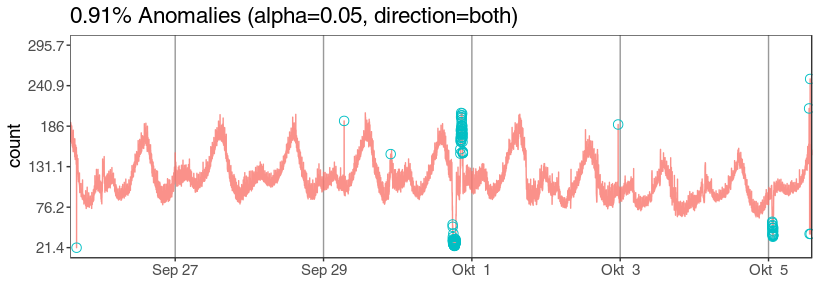
\includegraphics{imgPres/TS_anomalydetection.png}
  \href{https://github.com/twitter/AnomalyDetection}{source}
\item
  fill in missing values (interpolation)
\item
  regular time-step

  \begin{itemize}
  \tightlist
  \item
    smoothing
  \item
    decimate
  \end{itemize}
\end{itemize}

\end{frame}

\begin{frame}[fragile]{Time series - Dynamic visualisation}

Dynamic time series visualisation with package
\href{https://cran.r-project.org/web/packages/dygraph/index.html}{\texttt{dygraph}}

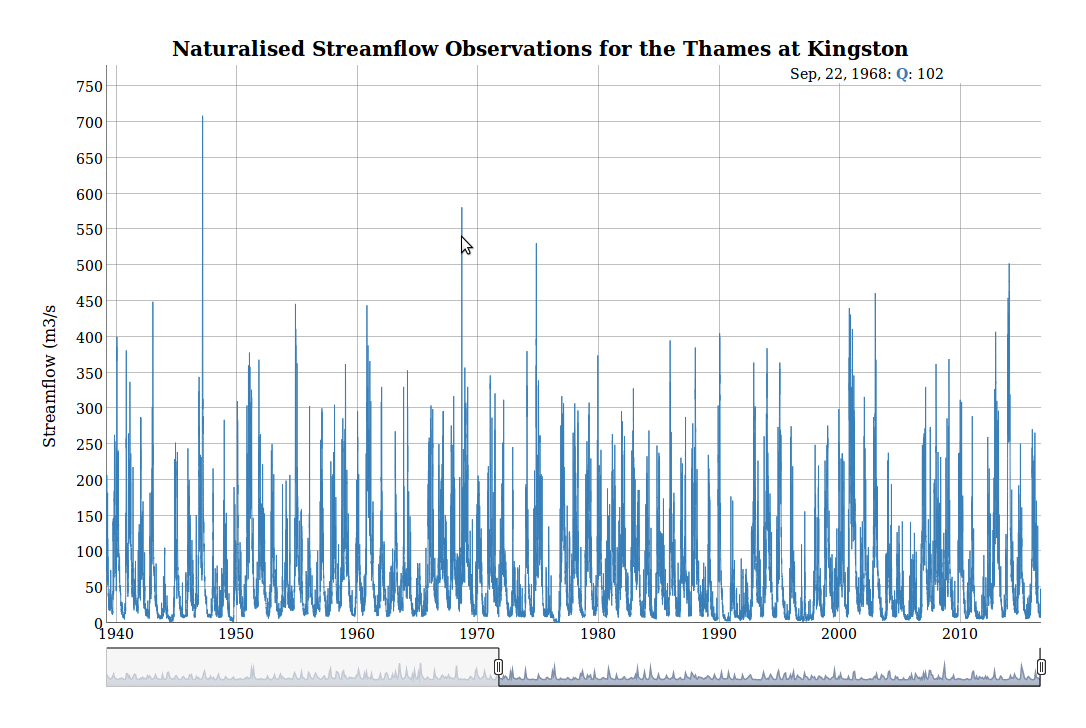
\includegraphics{imgPres/dygraph.png}

\end{frame}

\begin{frame}[fragile]{Time series - Visualisation}

merci MM!

Import of groundwater head data from FEFLOW

\texttt{P:/RKurs/...}
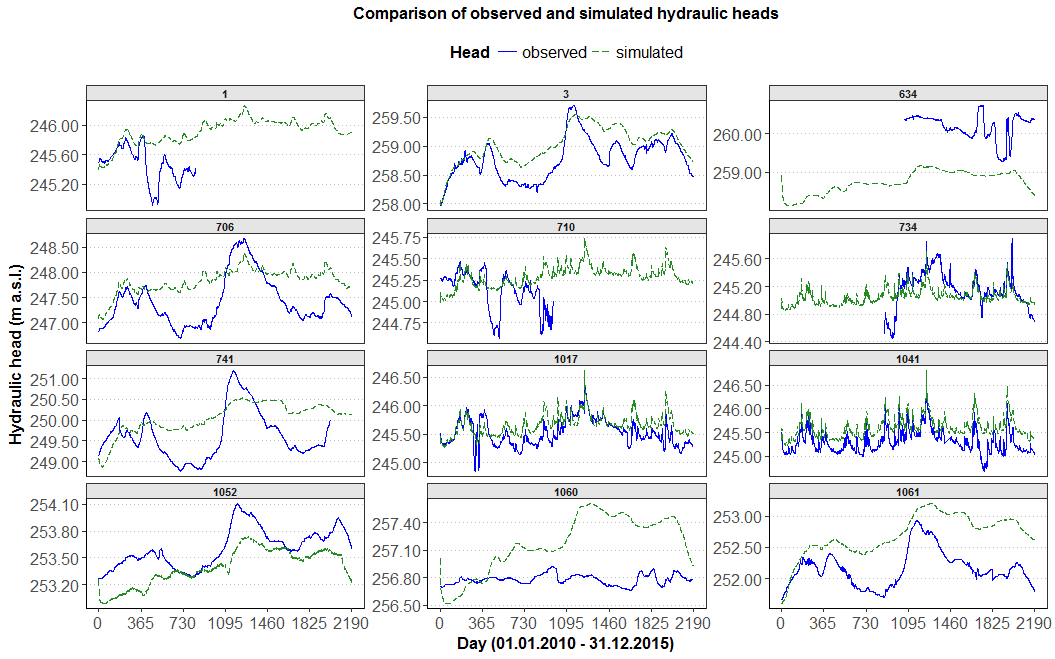
\includegraphics{imgPres/time_series_head_analysis01.png}

\end{frame}

\begin{frame}{Time series - Simulated vs observed}

\columnsbegin
\column{.5\textwidth}
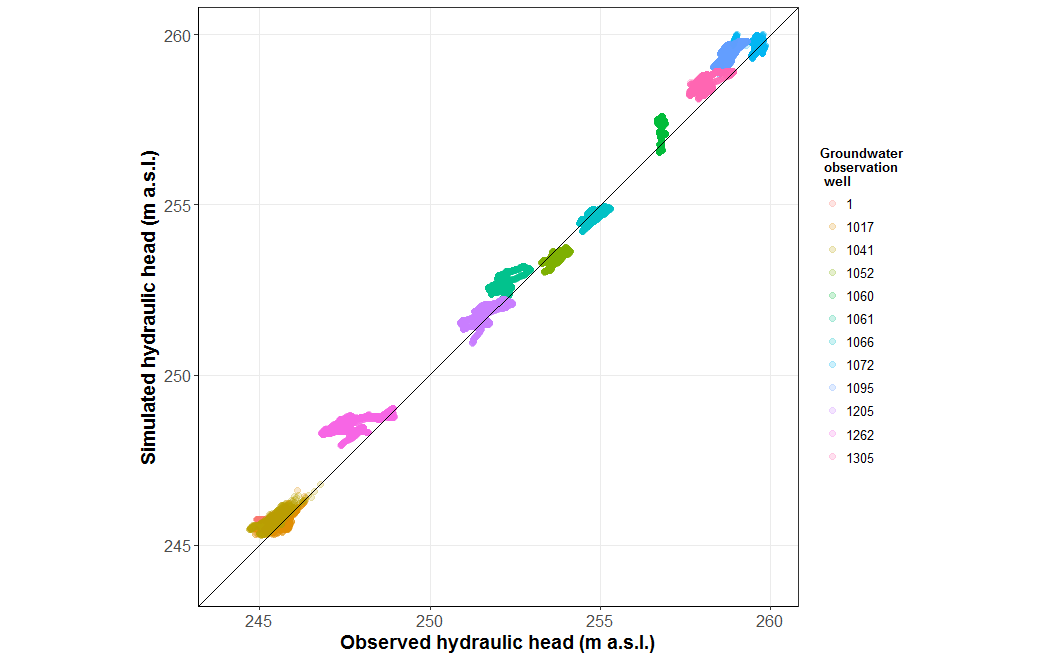
\includegraphics{imgPres/time_series_head_analysis02.png}
\column{.5\textwidth}
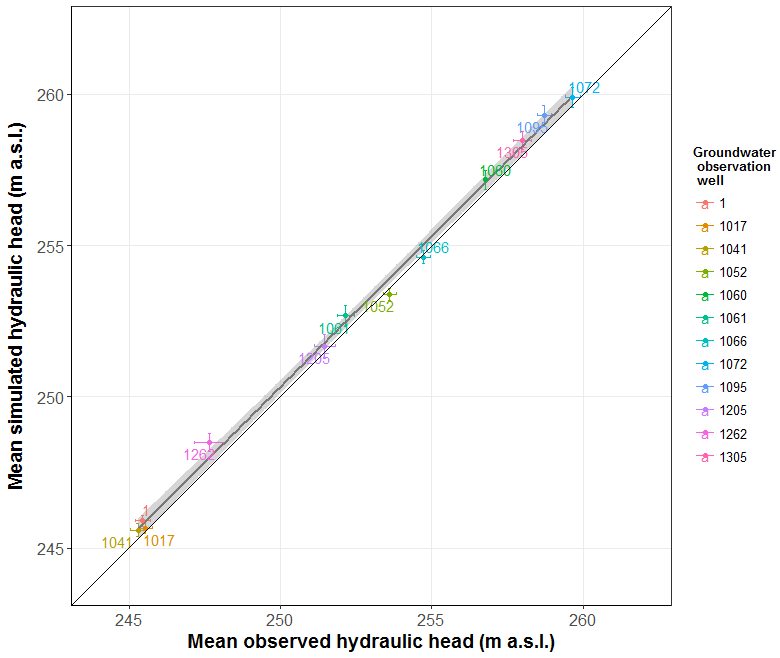
\includegraphics{imgPres/time_series_head_analysis03.png} \columnsend

\end{frame}

\begin{frame}{Time series - Goodness-of-fit}

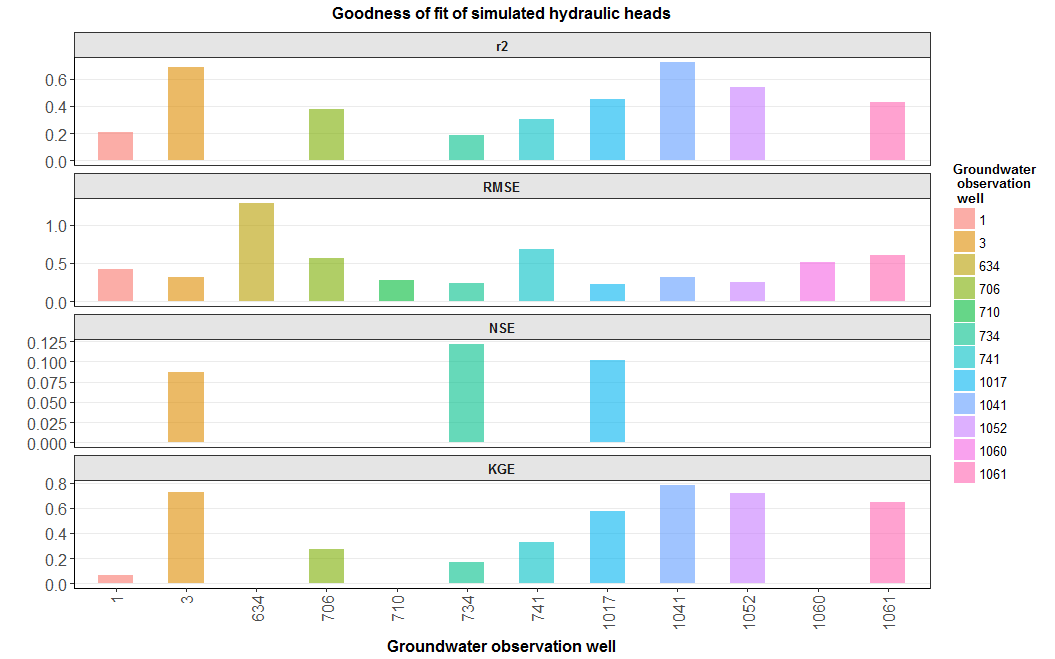
\includegraphics{imgPres/time_series_head_analysis04.png}

\end{frame}

\begin{frame}{Time series - Residual visualisation \emph{à la GMS}}

\columnsbegin
\column{.4\textwidth} 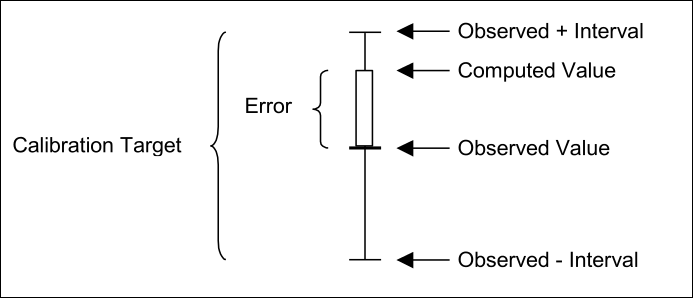
\includegraphics{imgPres/ts_residuals.png}
\column{.6\textwidth}
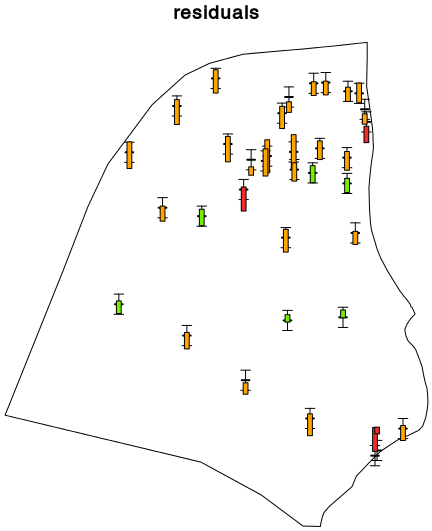
\includegraphics{imgPres/ts_resdiuals_examples.png} \columnsend

\end{frame}

\begin{frame}[fragile]{Time series - Clustering}

\columnsbegin
\column{.7\textwidth}

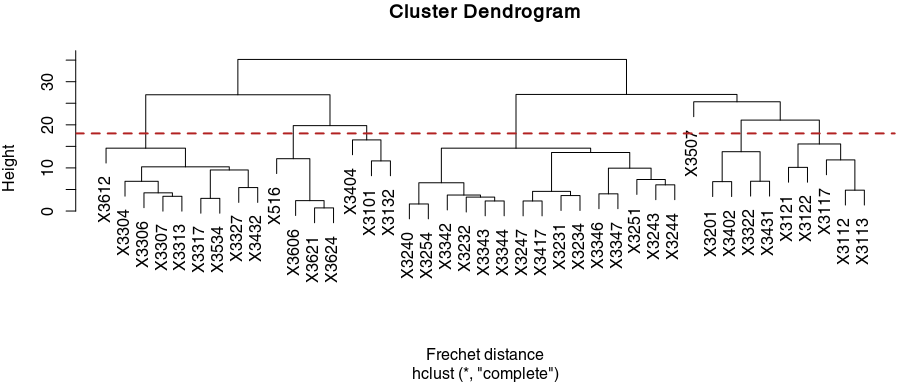
\includegraphics[width=0.90000\textwidth]{imgPres/ts_cluster_dendo.png}

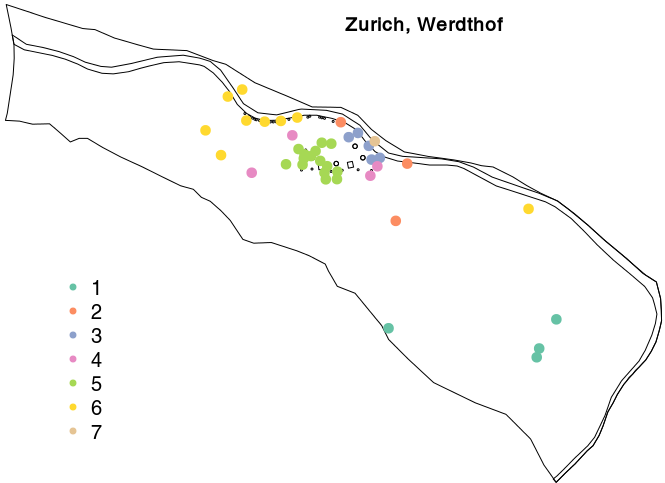
\includegraphics[width=0.80000\textwidth]{imgPres/ts_cluster_map.png}
\column{.3\textwidth}

\begin{itemize}
\tightlist
\item
  remove obs with too many \texttt{NA}'s
\item
  interpolate missing data \texttt{NA}
\item
  compute distances between obs
\item
  cut dendrogram --\textgreater{} classes
\item
  plot onto map
\end{itemize}

\columnsend

\end{frame}

\begin{frame}{Time series - statistics}

\begin{itemize}
\tightlist
\item
  Daily, monthly, yearly values (cf.~book: Analysis of ecological data
  with R)
\item
  Auto-correlation function (ACF) and Cross-correlation function (CCF)
  See ARIMA model
  \href{https://www.analyticsvidhya.com/blog/2015/12/complete-tutorial-time-series-modeling/}{tutorial},
  \href{http://a-little-book-of-r-for-time-series.readthedocs.io/en/latest/src/timeseries.html}{tutorial2}
\item
  empirical cumulative distribution function
\end{itemize}

\end{frame}

\begin{frame}{Time series - spectral analysis}

\begin{itemize}
\tightlist
\item
  Fourier
\item
  SSA
\item
  ?
\item
  wavelet analysis
\end{itemize}

\end{frame}

\begin{frame}{Time series - impulse response function}

Check RRAWFLOW package
\href{https://sd.water.usgs.gov/projects/RRAWFLOW/RRAWFLOW.html}{rrawflow
website}

\end{frame}

\begin{frame}{Time series - Interpolation}

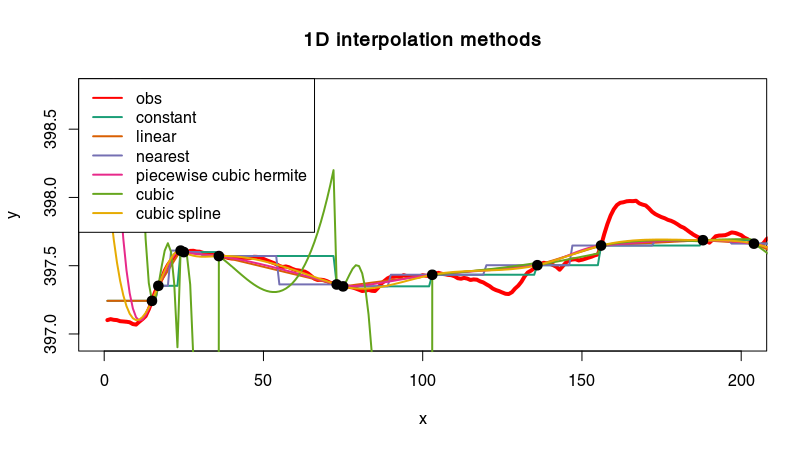
\includegraphics[height=0.35000\textwidth]{imgPres/TS_1D_interp.png}

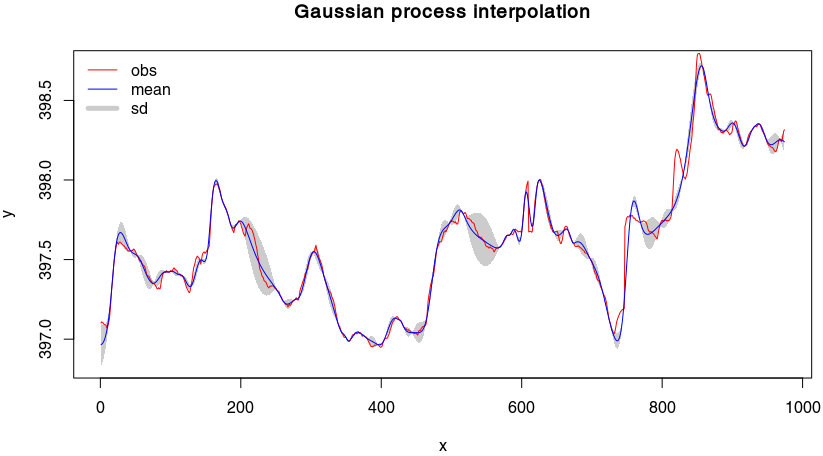
\includegraphics[height=0.35000\textwidth]{imgPres/TS_GP_interp.png}

\end{frame}

\begin{frame}{Time series - regression}

\begin{itemize}
\tightlist
\item
  Regression
\end{itemize}

\end{frame}

\begin{frame}[fragile]{Time series - Trend and seasonal components}

\columnsbegin
\column{.5\textwidth} 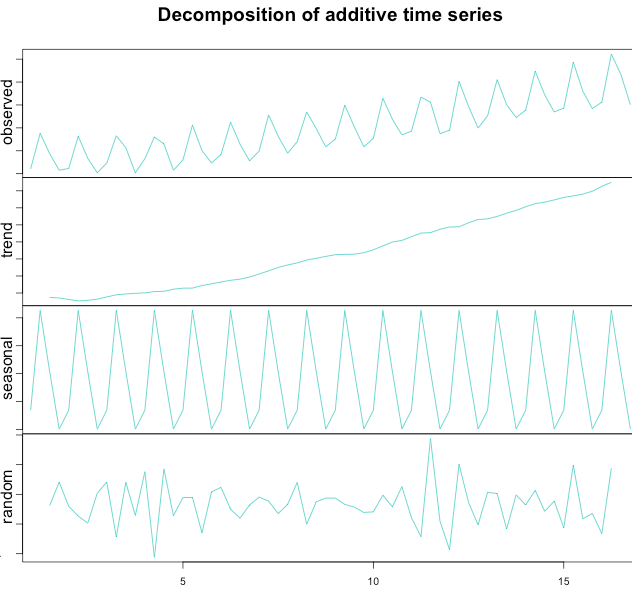
\includegraphics{imgPres/additive-decompose.png}
\column{.5\textwidth}
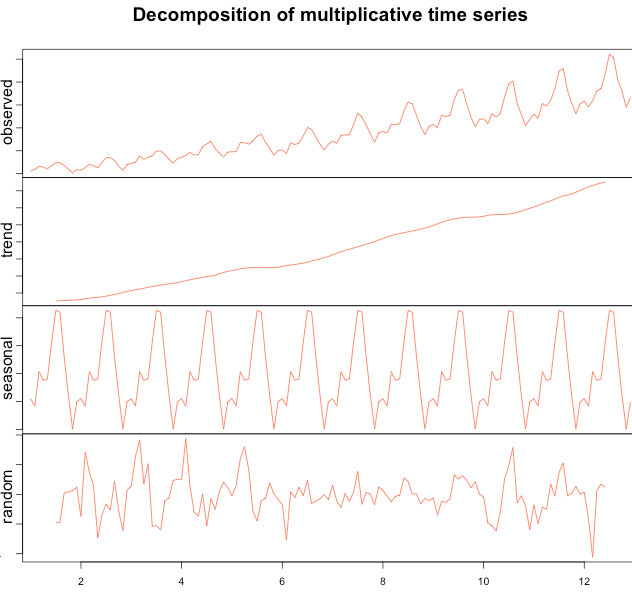
\includegraphics{imgPres/multiplicative-decompose.png} \columnsend

\begin{Shaded}
\begin{Highlighting}[]
\NormalTok{x_dcp_add <-}\StringTok{ }\KeywordTok{decompose}\NormalTok{(x, }\StringTok{"additive"}\NormalTok{)}
\NormalTok{x_dcp_mul <-}\StringTok{ }\KeywordTok{decompose}\NormalTok{(x, }\StringTok{"multiplicative"}\NormalTok{)}
\end{Highlighting}
\end{Shaded}

\href{https://anomaly.io/seasonal-trend-decomposition-in-r/}{online
tutorial}

\end{frame}

\begin{frame}{Time series - mining and clustering}

\href{https://rdatamining.wordpress.com/2011/08/23/time-series-analysis-and-mining-with-r/}{Time
series mining and clustering}

\begin{itemize}
\tightlist
\item
  Compute distance between time-series
\item
  Clustering
\item
  Vizualisation (e.g., MDS)
\end{itemize}

\end{frame}

\begin{frame}[fragile]{Time series - change detection}

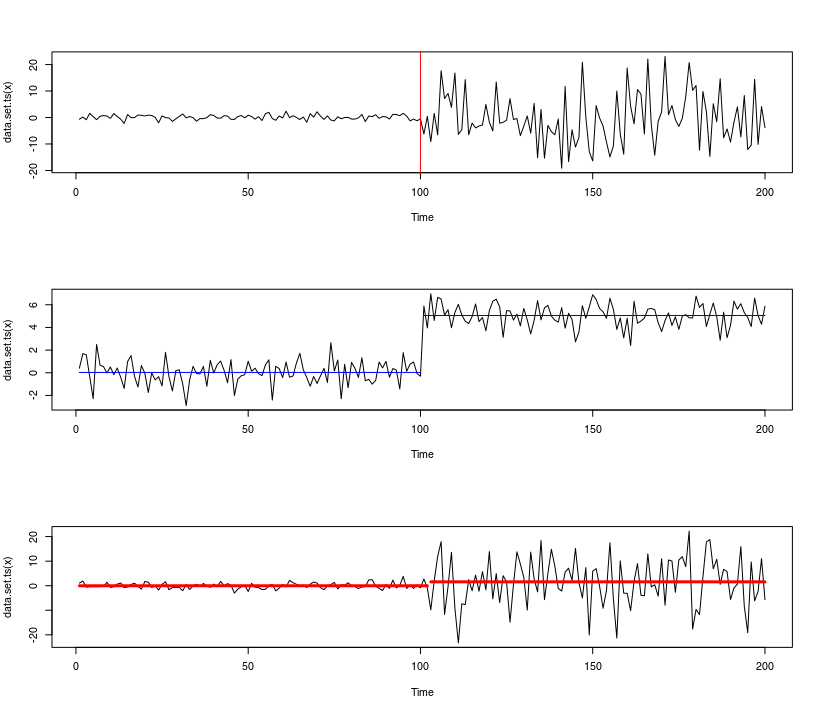
\includegraphics{imgPres/TS_changedetection.png} package
\href{https://cran.r-project.org/web/packages/changepoint}{\texttt{changepoint}}

\begin{itemize}
\tightlist
\item
  Example: NF-Fisch Plot CP1 against CP2 and CP3: ellipses
\item
  CD-Experiment
\item
  Gaussian process (\texttt{GauProMod})
\item
  \href{https://cran.r-project.org/web/packages/waterData/vignettes/vignette.pdf}{time-series
  cleanup}
\item
  \href{http://www.css.cornell.edu/faculty/dgr2/teach/R/R_ts.pdf}{time-series}
\end{itemize}

\end{frame}

\begin{frame}[fragile]{R GIS - resources}

\href{ftp://ftp.bgc-jena.mpg.de/pub/outgoing/mforkel/Rcourse/spatialR_2015.pdf}{R
is a GIS software} (sp, rgeos, raster, rgdal) see also \texttt{sf} :
\href{https://cran.r-project.org/web/packages/sf/vignettes/sf1.html}{chjeck}

\begin{itemize}
\tightlist
\item
  \textbf{Package}

  \begin{itemize}
  \tightlist
  \item
    \href{https://cran.r-project.org/web/packages/sf/index.html}{\texttt{sf}}
    package for spatial vector data. Binds to GDAL for reading and
    writing data, to GEOS for geometrical operations, and to Proj.4 for
    projection conversions and datum (\emph{will remplace sp/rgeos/rgdal
    in the long term}
    \href{https://github.com/r-spatial/sf/wiki/migrating}{link})
  \item
    \href{https://cran.r-project.org/web/packages/raster/index.html}{\texttt{raster}}
    package for raster, multi-band raster, \ldots{}
  \item
    \href{https://github.com/Jean-Romain/lidR}{lidR} for airborne LiDAR
    data manipulation and visualization for forestry application
  \item
    packages to interact with existing GIS software
    \href{http://jwhollister.com/r_landscape_tutorial/tutorial.html}{link}

    \begin{itemize}
    \tightlist
    \item
      \texttt{spgrass6}: Provides an interface between R and GRASS 6+.
      Allows for running R from within GRASS as well as running GRASS
      from within R.
    \item
      \texttt{rgrass7}: Same as spgrass6, but for the latest version of
      GRASS, GRASS 7.
    \item
      \texttt{RPyGeo}: A wrapper for accessing ArcGIS from R. Utilizes
      intermediate python scripts to fire up ArcGIS. Hasn't been updated
      in some time.
    \item
      \texttt{RSAGA}: R interface to the command line version of SAGA
      GIS.
    \end{itemize}
  \end{itemize}
\item
  \textbf{Cheat sheet}

  \begin{itemize}
  \tightlist
  \item
    nothing\ldots{}
  \end{itemize}
\item
  \textbf{Tutorials/book}

  \begin{itemize}
  \tightlist
  \item
    \href{https://bookdown.org/robinlovelace/geocompr}{Book:
    geocomputation with R}
  \item
    \href{http://rspatial.org/intr/index.html}{Spatial Data Analysis and
    Modeling with R}
  \end{itemize}
\end{itemize}

\end{frame}

\begin{frame}{R GIS}

\columnsbegin

\column{.4\textwidth}

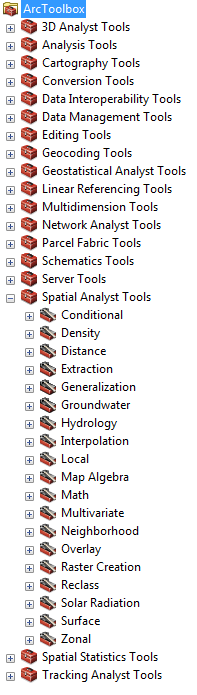
\includegraphics{imgPres/R_is_a_GIS.png}

\column{.6\textwidth}

\textbf{Tool}

\begin{itemize}
\tightlist
\item
  manipulation raster
\item
  manipulation feature
\item
  raster interpolation:

  \begin{itemize}
  \tightlist
  \item
    book: R\_Applied Spatial Data Analysis with R.pdf (chap. 8, 8.11)
  \end{itemize}
\end{itemize}

\textbf{Still missing}

\begin{itemize}
\tightlist
\item
  TIN
\item
  watershed but

  \begin{itemize}
  \tightlist
  \item
    check
    \href{https://gis.stackexchange.com/questions/182120/get-rivers-from-a-dem-raster}{that}
  \item
    check
    \href{https://gis.stackexchange.com/questions/84309/what-algorithm-is-used-by-arcgis-watershed-tool}{how
    to compute flow accumulation}
  \item
    idea: use local structure tensor to compute direction and
    accumulation\ldots{}.
  \end{itemize}
\item
  download tiles webgis of Italy region
\end{itemize}

\columnsend

\end{frame}

\begin{frame}{R GIS - DEM processing}

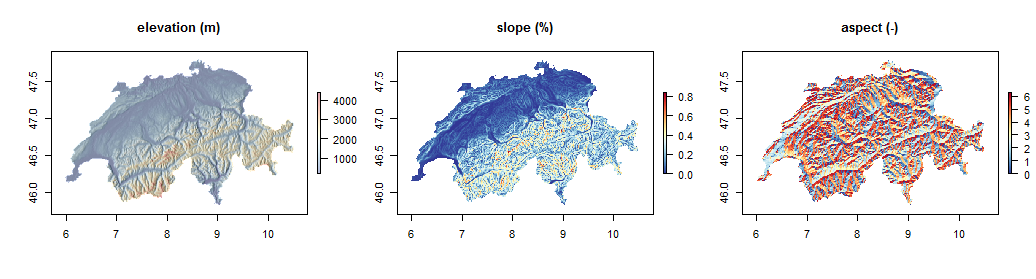
\includegraphics{imgPres/R_GIS01.png}

\end{frame}

\begin{frame}{R GIS - Feature projection}

\href{http://r-spatial.org/r/2017/01/12/newssf.html}{check graticules sf
class}

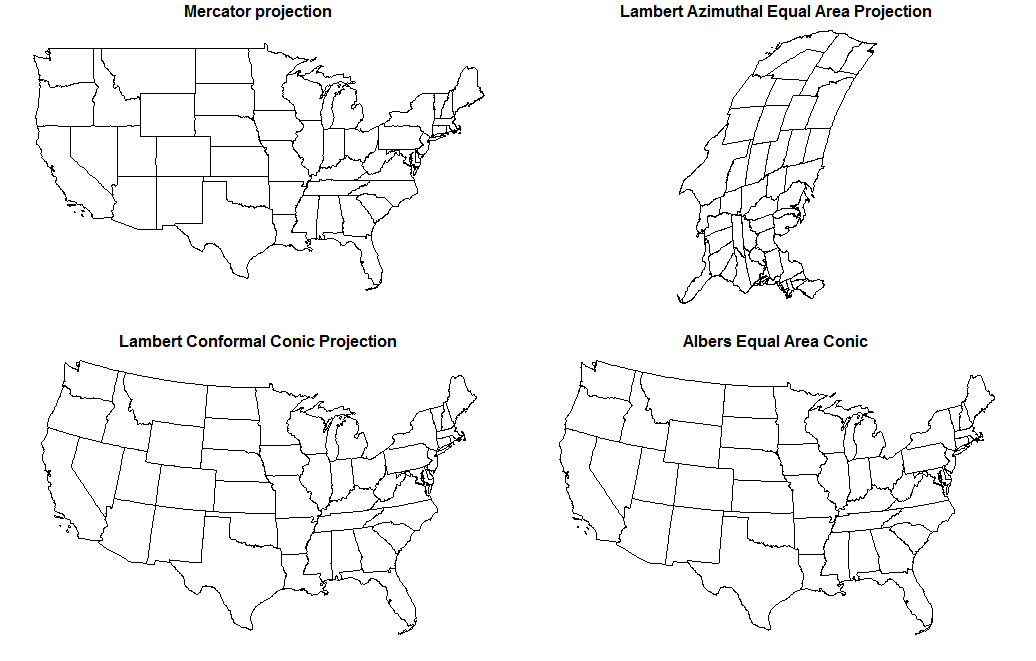
\includegraphics{imgPres/R_GIS_projection.png}

\end{frame}

\begin{frame}{R GIS - Maps (1)}

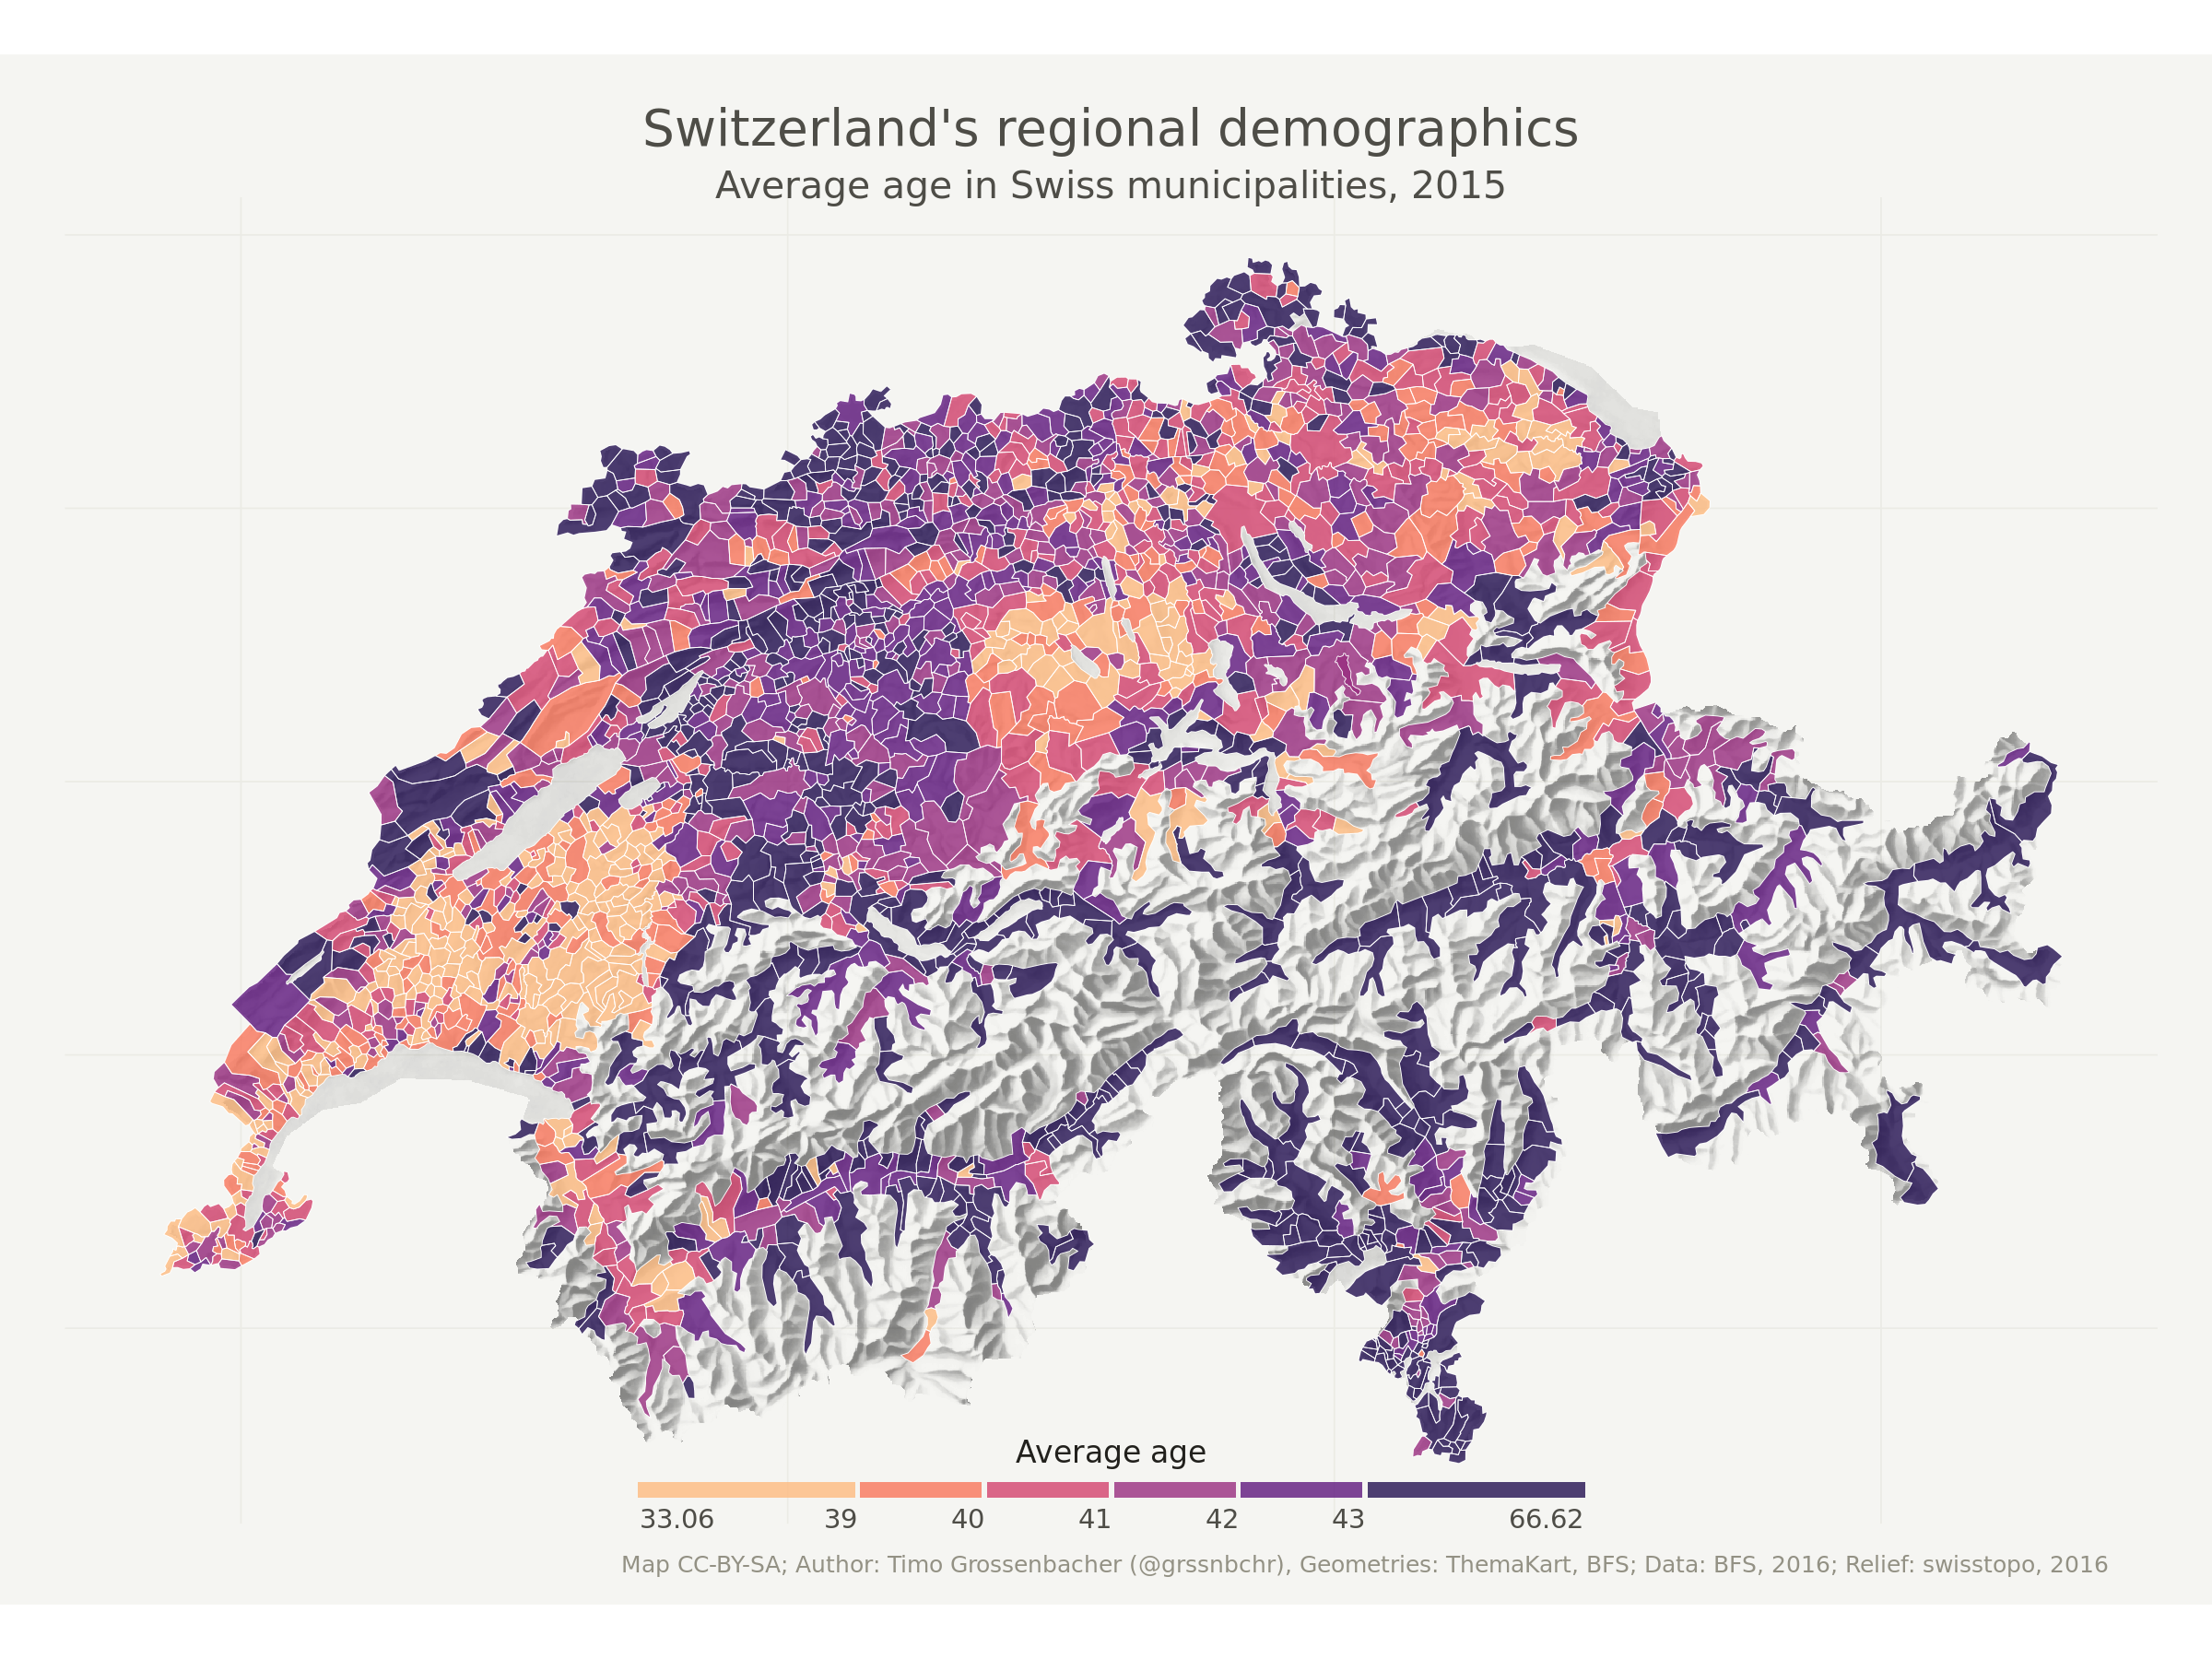
\includegraphics{imgPres/demo/R_as_a_GIS.png}
\href{https://timogrossenbacher.ch/2016/12/beautiful-thematic-maps-with-ggplot2-only/}{link}

\end{frame}

\begin{frame}{R GIS - Map (2)}

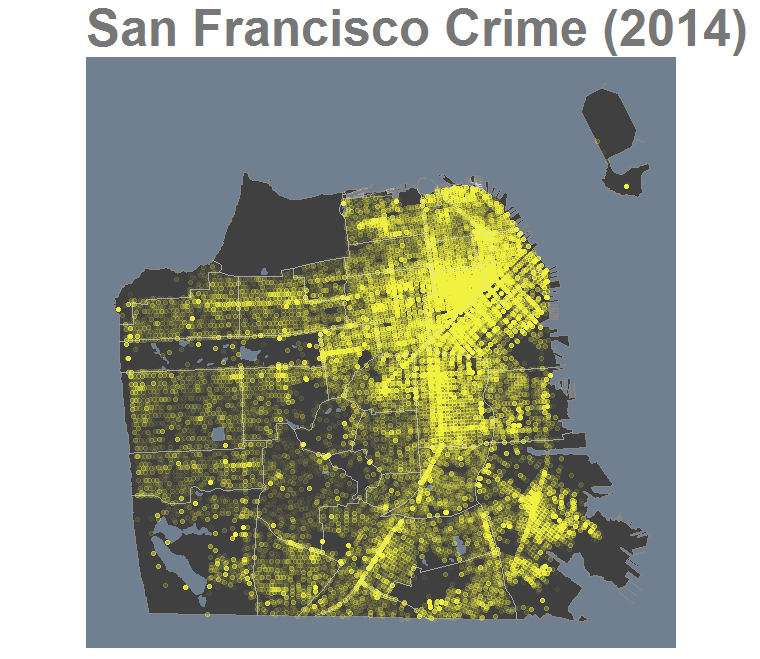
\includegraphics{imgPres/map_SF_Crime2014.png}
\href{http://sharpsightlabs.com/blog/mapping-san-francisco-crime/}{link}

\end{frame}

\begin{frame}[fragile]{R GIS - Spatial interpolation}

Raster interpolation \columnsbegin
\column{.4\textwidth} Adapted from
\href{http://rspatial.org/analysis/rst/4-interpolation.html}{here} and
\href{https://mgimond.github.io/Spatial/interpolation-in-r.html\#st-order-polynomial-fit}{here}
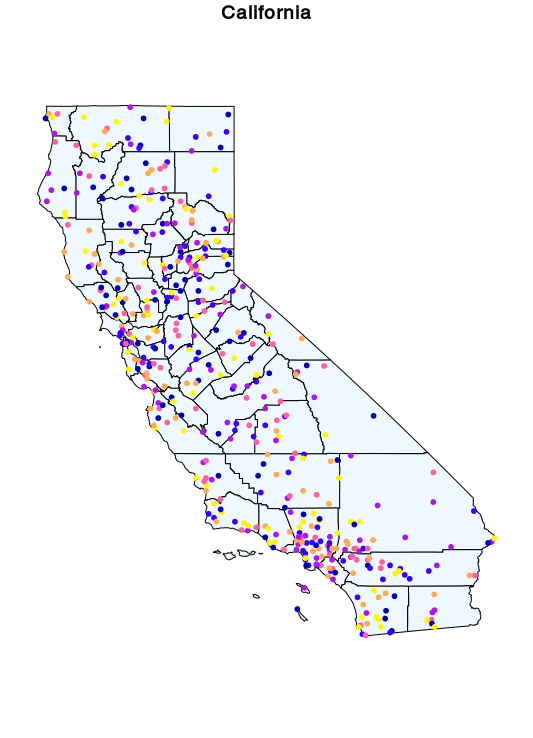
\includegraphics{imgPres/GIS_raster_interp_data.png}
\column{.6\textwidth} 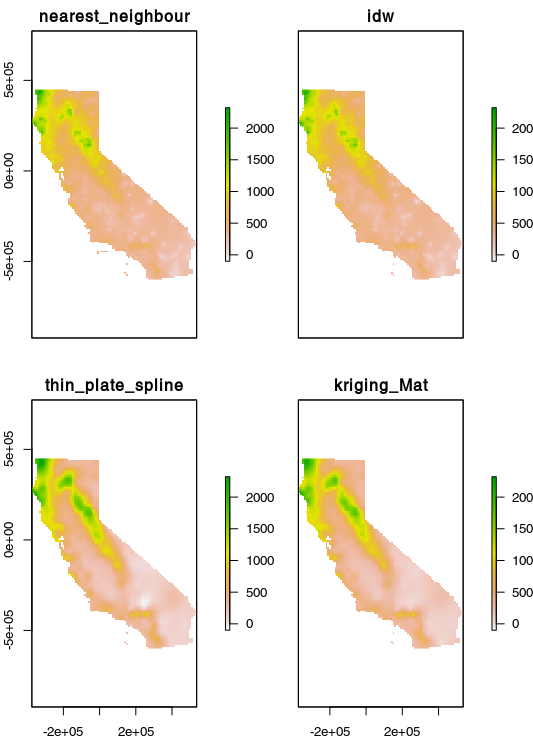
\includegraphics{imgPres/GIS_spatial_interp.png}
\columnsend

See also -
\href{https://cran.r-project.org/web/packages/ipdw/vignettes/ipdw2.html}{\texttt{ipdw}
Spatial Interpolation via Inverse Path Distance Weighting} -
\href{https://mgimond.github.io/Spatial/interpolation-in-r.html}{check
that}

\end{frame}

\begin{frame}{R GIS - LiDAR}

R package for airborne LiDAR data manipulation and visualisation for
forestry application \href{https://github.com/Jean-Romain/lidR}{lidR}

\end{frame}

\begin{frame}{R GIS - making and using bathymetric maps in R with
\texttt{marmap}}

\href{https://www.ncbi.nlm.nih.gov/pmc/articles/PMC3760912/}{link}

\end{frame}

\begin{frame}[fragile]{Image analysis and processing - resources}

\begin{itemize}
\tightlist
\item
  \textbf{Package}

  \begin{itemize}
  \tightlist
  \item
    \href{https://cran.r-project.org/web/packages/imager/index.html}{\texttt{imager}}
  \item
    \href{https://cran.r-project.org/web/packages/EBImage/index.html}{\texttt{EBImage}}
  \end{itemize}
\item
  \textbf{Tutorials/book}

  \begin{itemize}
  \tightlist
  \item
    \href{https://cran.r-project.org/web/packages/imager/index.html}{check
    \texttt{imager} vignettes}
  \item
    \href{https://dahtah.github.io/imager/}{\texttt{imager} project
    website}
  \item
    \href{https://www.bioconductor.org/packages/3.7/bioc/vignettes/EBImage/inst/doc/EBImage-introduction.html}{check
    \texttt{EBImage} vignettes}
  \end{itemize}
\end{itemize}

\end{frame}

\begin{frame}[fragile]{Image analysis and processing}

Example: package \texttt{imager}
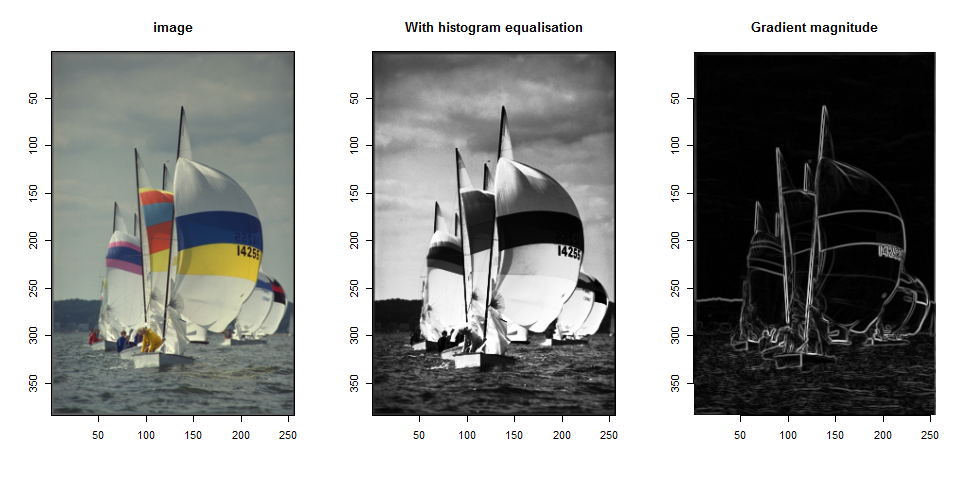
\includegraphics{imgPres/image_processing.png}

\end{frame}

\begin{frame}{GPR data processing \texttt{RGPR} (1)}

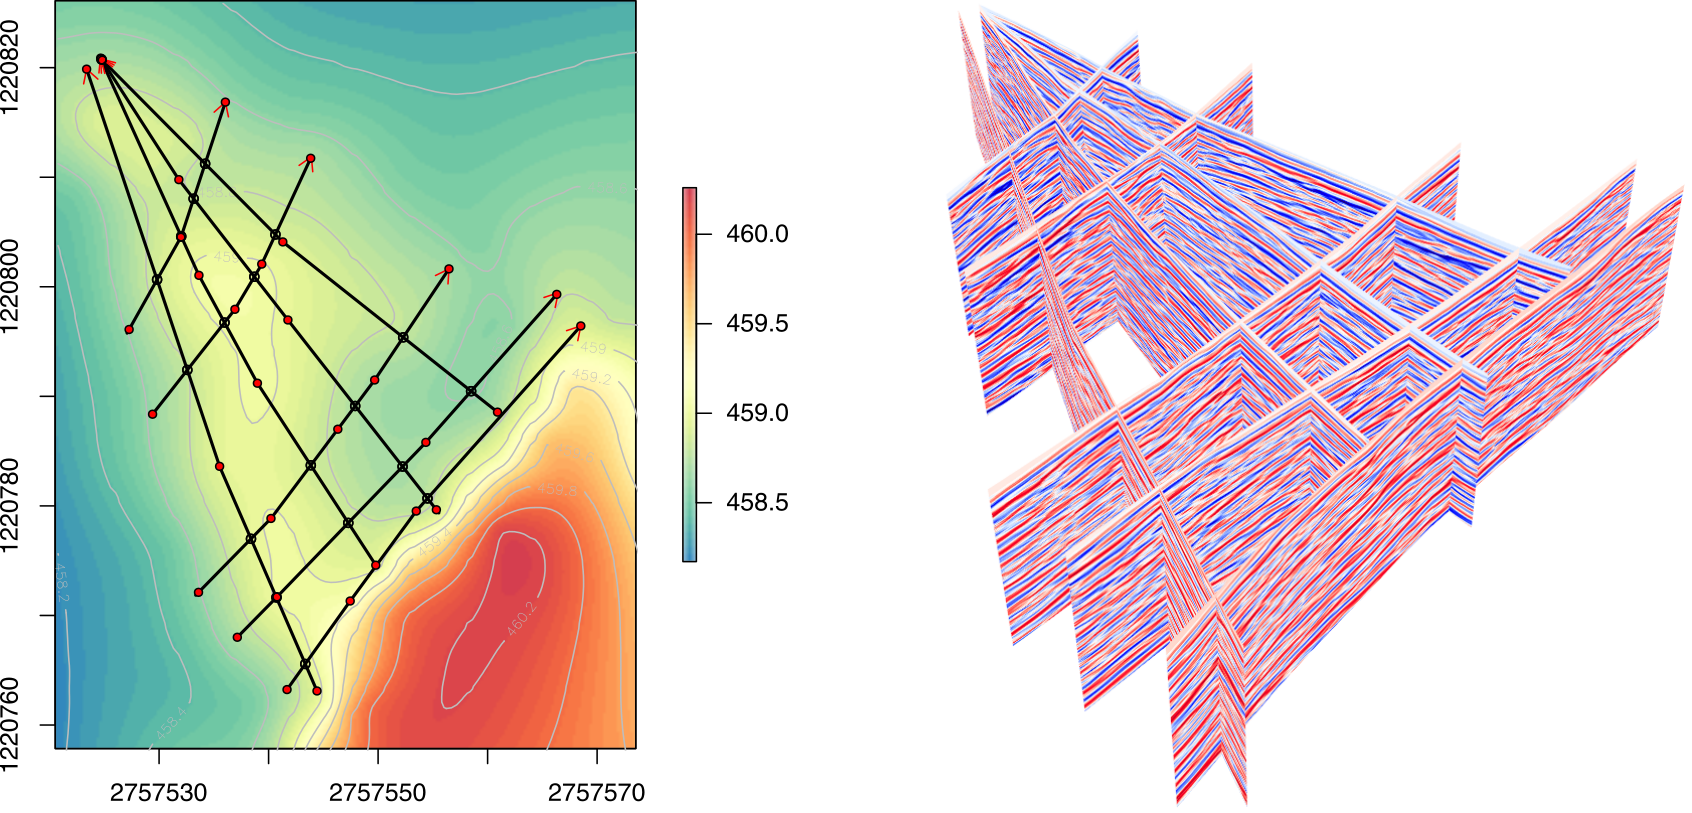
\includegraphics{imgPres/GPR_processing01.png}

\end{frame}

\begin{frame}{GPR data processing \texttt{RGPR} (2)}

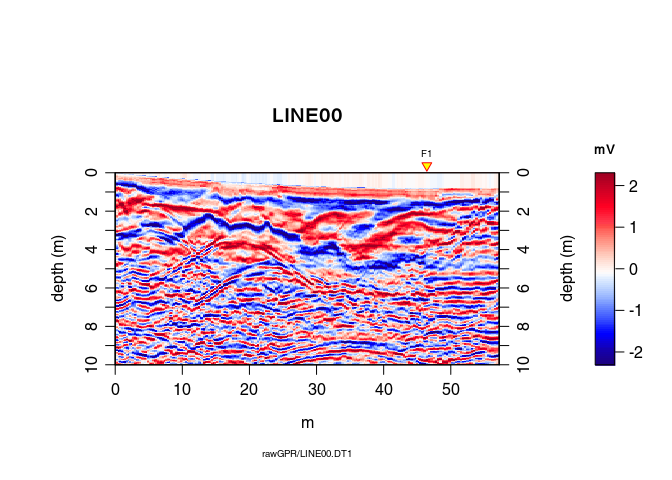
\includegraphics{imgPres/GPR_processing02.png}
\href{https://github.com/emanuelhuber/RGPR}{package}
\href{http://emanuelhuber.github.io/RGPR/}{tutorial}

\end{frame}

\begin{frame}{Seismic data}

\begin{itemize}
\tightlist
\item
  \href{http://mazamascience.com/Classes/IRIS_2015/}{seimic data
  analysis and processing}
\item
  \href{https://www.earth-surf-dynam-discuss.net/esurf-2017-75/esurf-2017-75.pdf}{eisis
  package}

  \begin{itemize}
  \tightlist
  \item
    \href{http://www.unc.edu/~leesj/FETCH/GRAB/Vignettes/whyRbeam.pdf}{talk}
  \end{itemize}
\end{itemize}

\end{frame}

\begin{frame}{Database}

\begin{itemize}
\item
  quality control: detect ``outliers'', bad quality data, errors
\item
  statistics, plots, reporting
\item
  \href{https://paulhcleverley.com/2017/05/28/text-analytics-meets-geoscience/}{text
  analytic meet geosciences}

  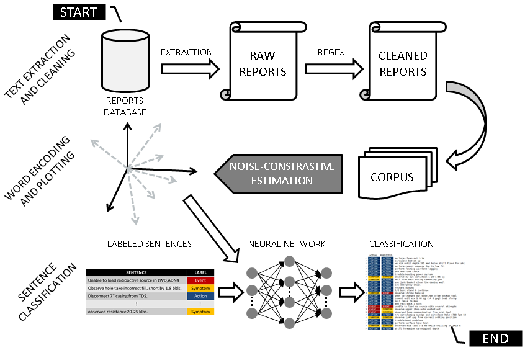
\includegraphics[width=0.50000\textwidth]{imgPres/text_analyse_drilling_report.png}

  from \href{https://arxiv.org/abs/1712.01476}{arxiv.org/abs/1712.01476}
\item
  Regli et al. (2002) Interpretation of drill core and georadar data of
  coarse gravel deposits
  \href{https://doi.org/10.1016/S0022-1694(01)00531-5}{doi:10.1016/S0022-1694(01)00531-5}
\end{itemize}

\end{frame}

\begin{frame}[fragile]{Misc}

\begin{itemize}
\tightlist
\item
  Package
  \href{https://cran.r-project.org/web/packages/rioja/}{\texttt{rioja}}:
  Functions for the analysis of Quaternary science data, including
  constrained clustering, WA, WAPLS, IKFA, MLRC and MAT transfer
  functions, and stratigraphic diagrams.
\end{itemize}

\end{frame}

\section{Modeling/simulations}\label{modelingsimulations}

\begin{frame}[fragile]{Statistical/stochastic models}

\begin{itemize}
\tightlist
\item
  probabilty distribution
\item
  Gaussian process/Kriging (\texttt{RandomFields}): account for
  correlation

  \begin{itemize}
  \tightlist
  \item
    3D subsurface heterogeneity model
  \end{itemize}
\item
  point process and marked point process

  \begin{itemize}
  \tightlist
  \item
    faults, \texttt{CBRDM}
  \end{itemize}
\end{itemize}

\end{frame}

\begin{frame}[fragile]{Catchment flow simulation}

\begin{itemize}
\tightlist
\item
  \texttt{RRAWFLOW}: Rainfall-Response Aquifer and Watershed Flow Model
\item
  \texttt{topmodel} and \texttt{dynatopmodel} packages
\end{itemize}

\end{frame}

\begin{frame}[fragile]{Catchment flow simulation (1)}

Package
\href{https://cran.r-project.org/web/packages/airGR/index.html}{\texttt{airGR}},
see tutorial on
\href{https://odelaigue.github.io/airGR/index.html}{companion website}

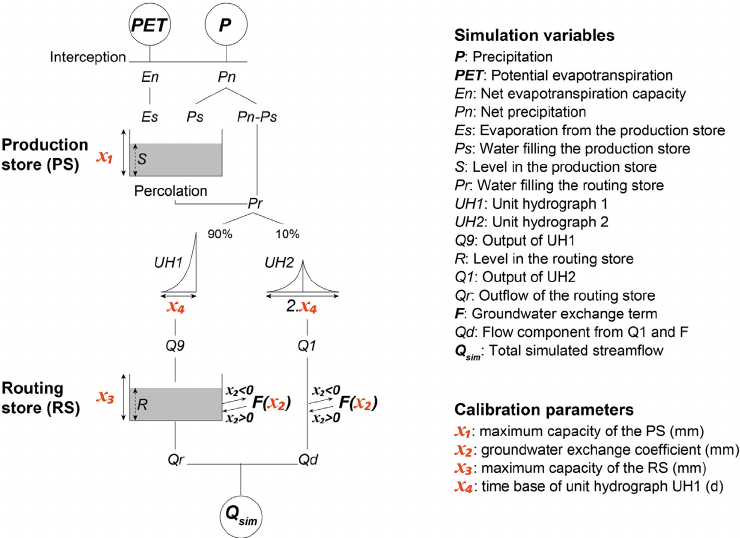
\includegraphics{imgPres/airGR_GR4J.png}

\end{frame}

\begin{frame}[fragile]{Catchment flow simulation (2)}

Package
\href{https://cran.r-project.org/web/packages/airGR/index.html}{\texttt{airGR}},
see \href{https://odelaigue.github.io/airGR/index.html}{companion
website}

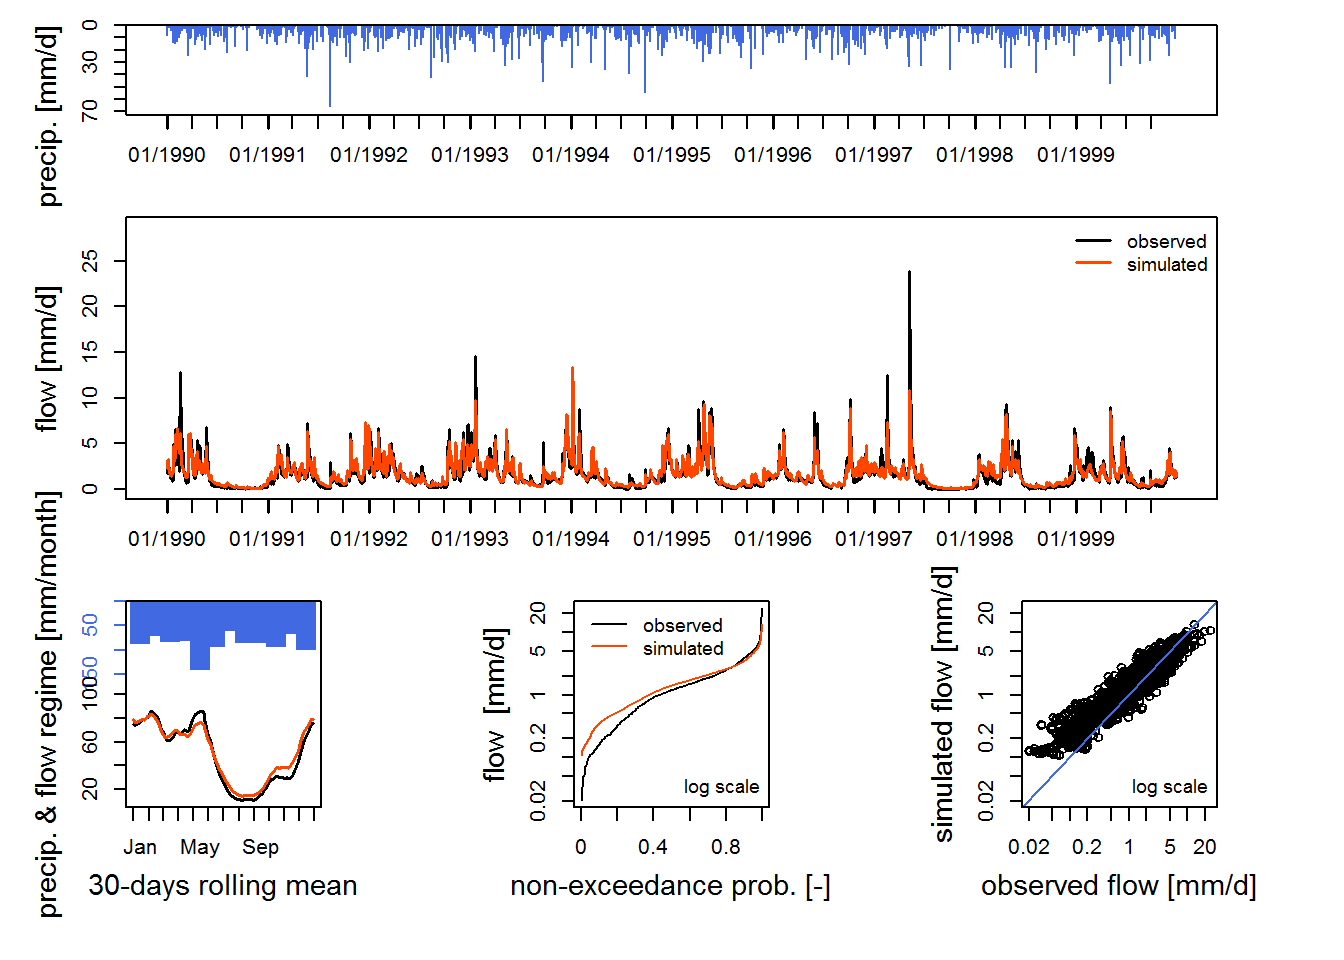
\includegraphics{imgPres/airGR.png}

\end{frame}

\begin{frame}[fragile]{Groundwater head interpolation}

package \texttt{GauProMod}: Gaussian process (Kriging) with constraints
on boundaries

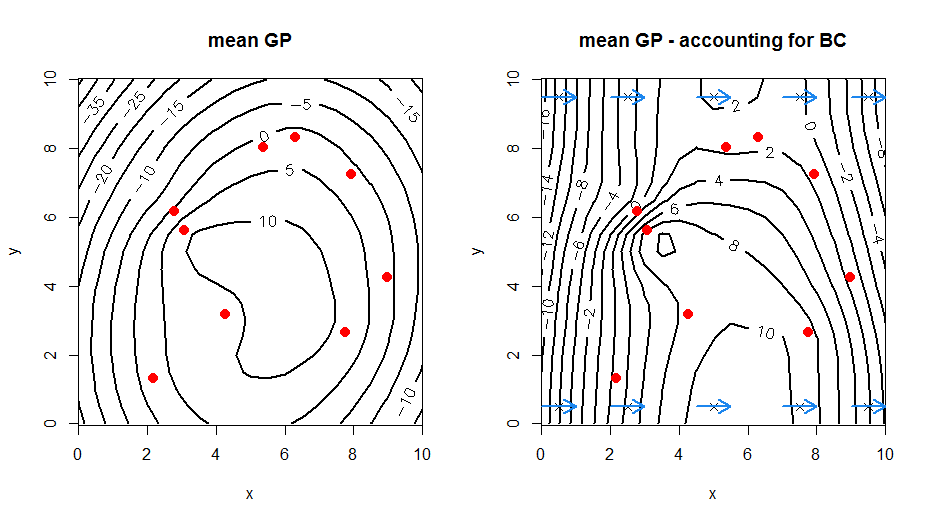
\includegraphics{imgPres/GP_head_interpolation.png}

After \href{https://doi.org/10.1016/j.jhydrol.2010.01.002}{Kuhlman and
Igusquiza (2010)}

\end{frame}

\begin{frame}{Modflow - US-GS reproducible report}

\href{https://github.com/USGS-R/wrv}{github.com/USGS-R/wrv}

\end{frame}

\begin{frame}{Modflow - subsurface flow mixing (1)}

personal code based
\href{https://github.com/USGS-R/wrv}{github.com/USGS-R/wrv}
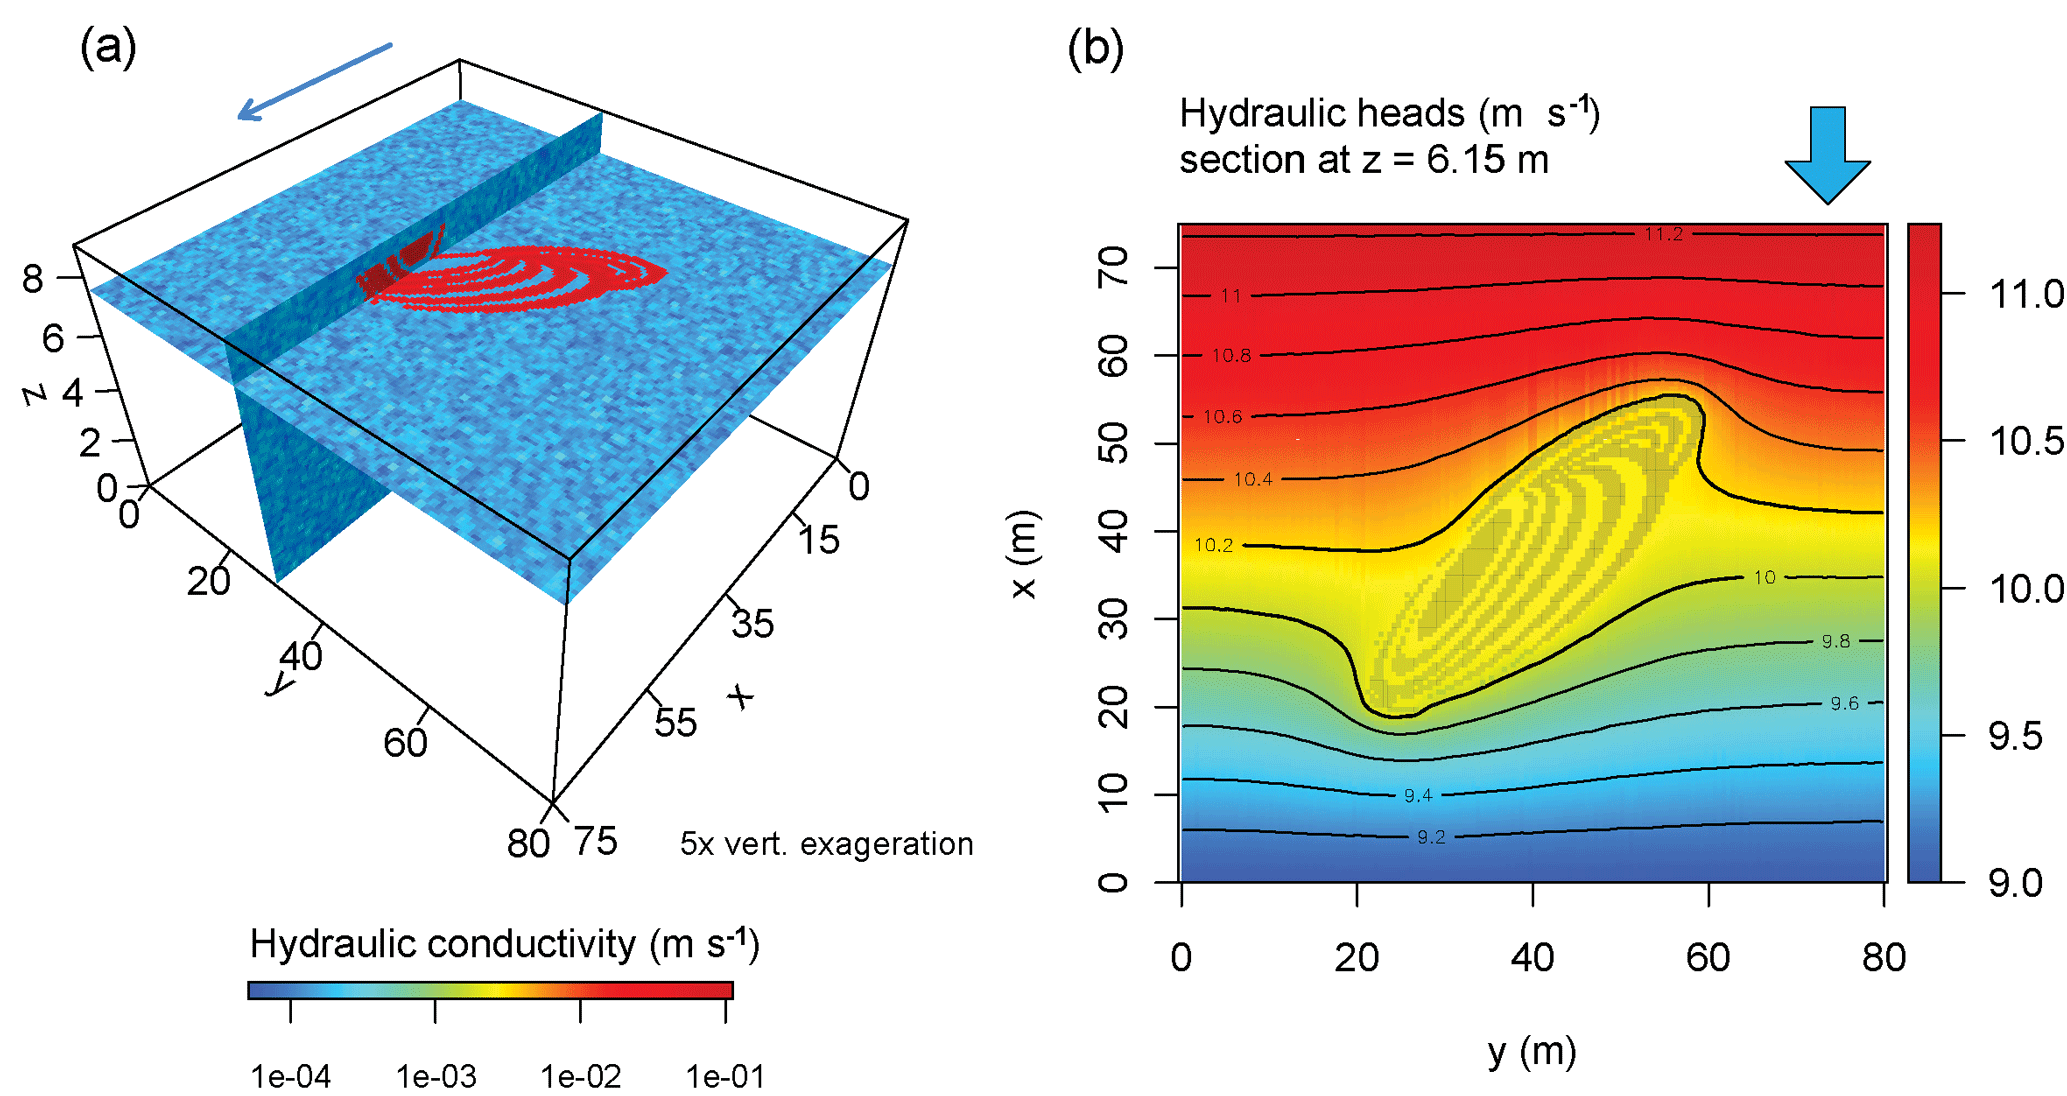
\includegraphics{imgPres/RMODFLOW_head.png}

\end{frame}

\begin{frame}{Modflow - subsurface flow mixing (2)}

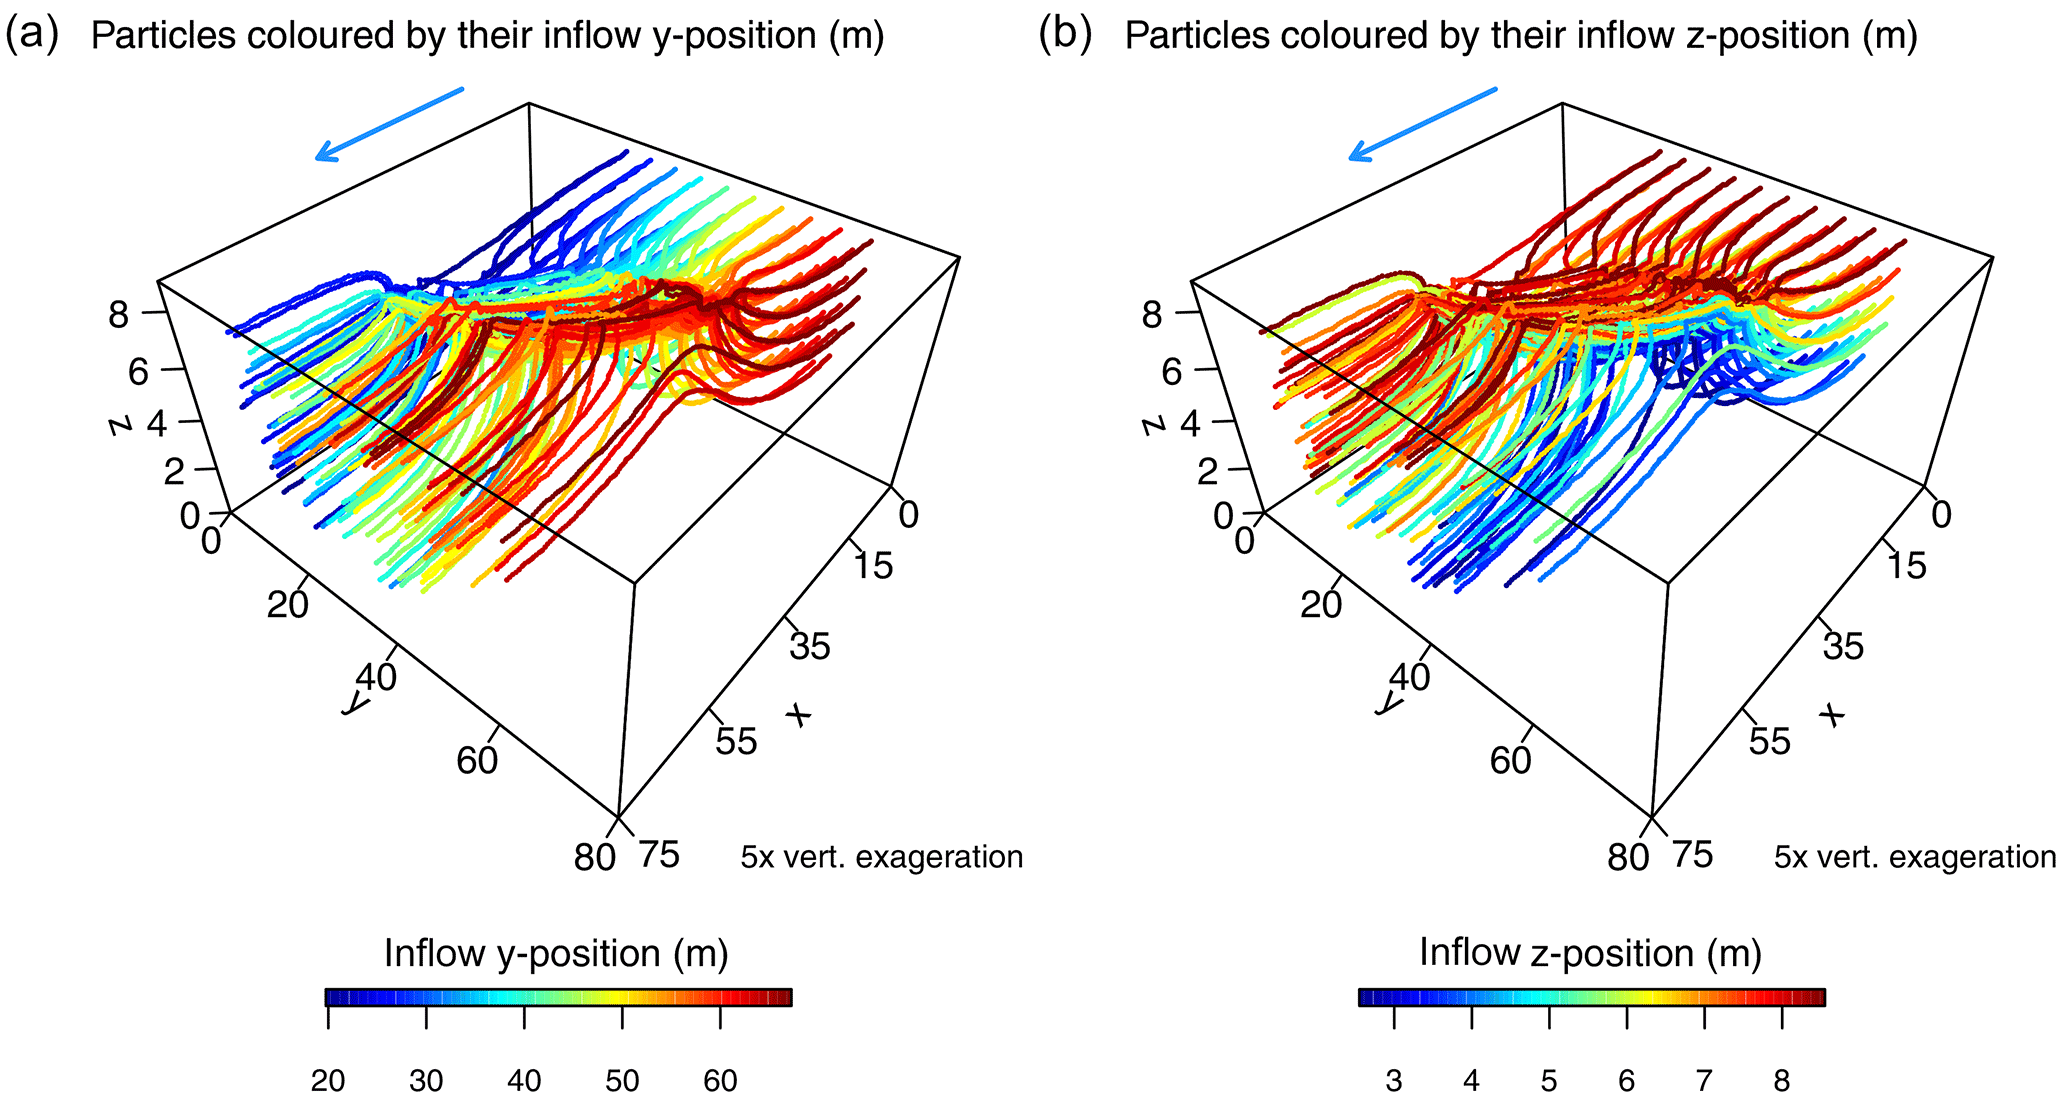
\includegraphics{imgPres/RMODFLOW_particles.png}

\end{frame}

\begin{frame}{Modflow - subsurface flow mixing (3)}

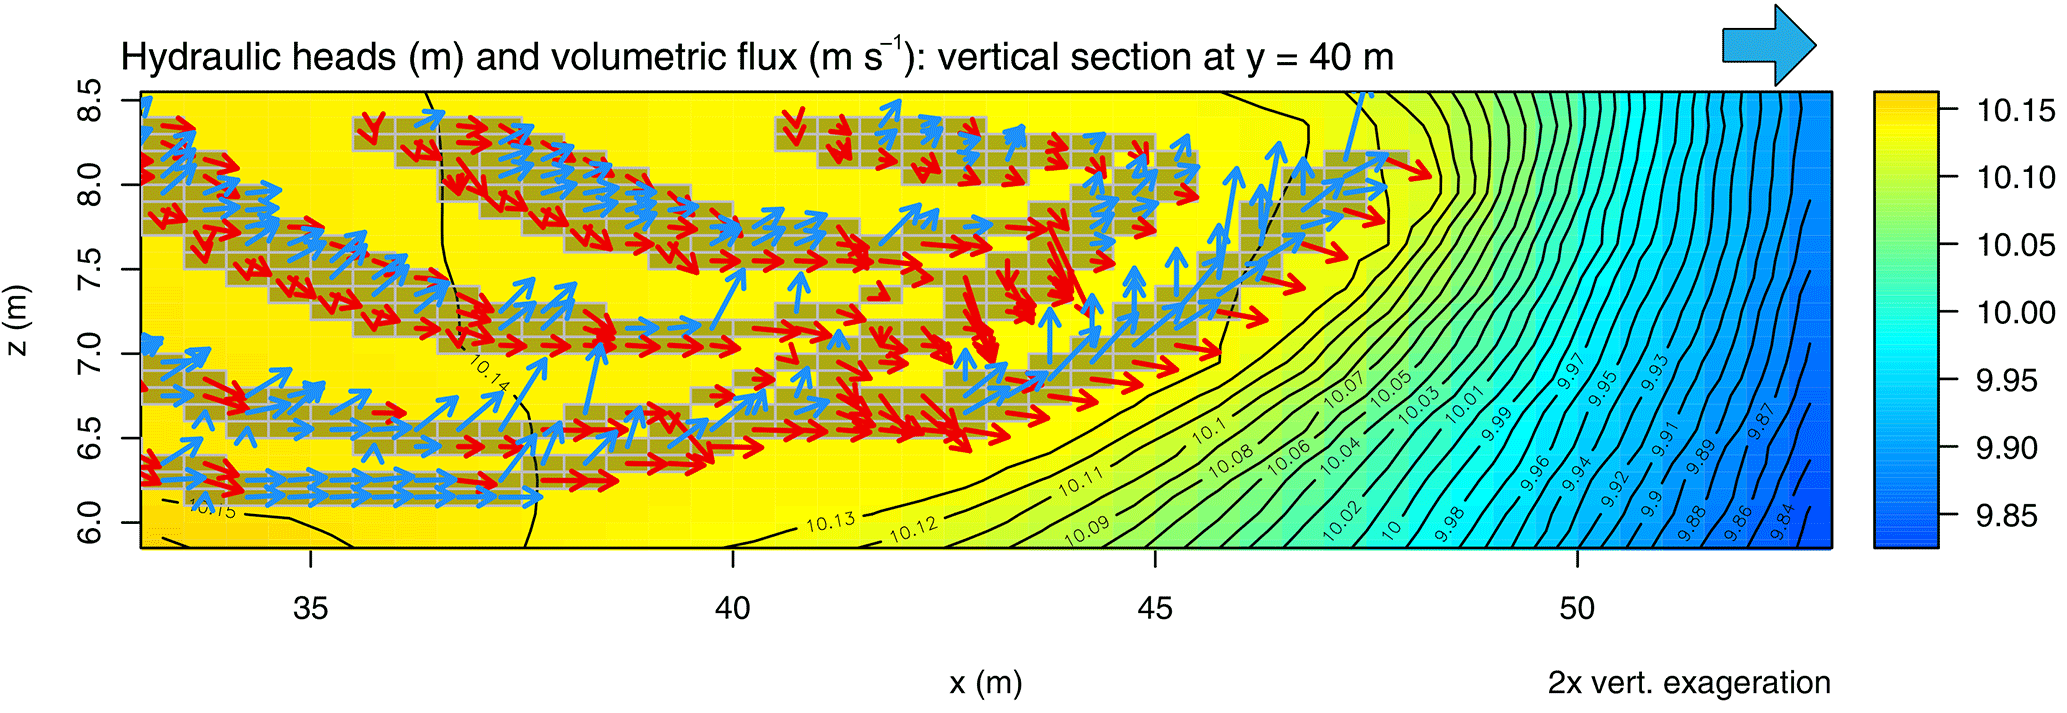
\includegraphics{imgPres/RMODFLOW_zoom.png}

\end{frame}

\begin{frame}[fragile]{Modflow -stochastic simulation (1)}

(\texttt{gwModBac} personal code based on
\href{https://github.com/USGS-R/wrv}{github.com/USGS-R/wrv} Groundwater
flow simulation and particle tracking to forecast microbial
concentration in a drinking water extraction well.

\begin{block}{Workflow}

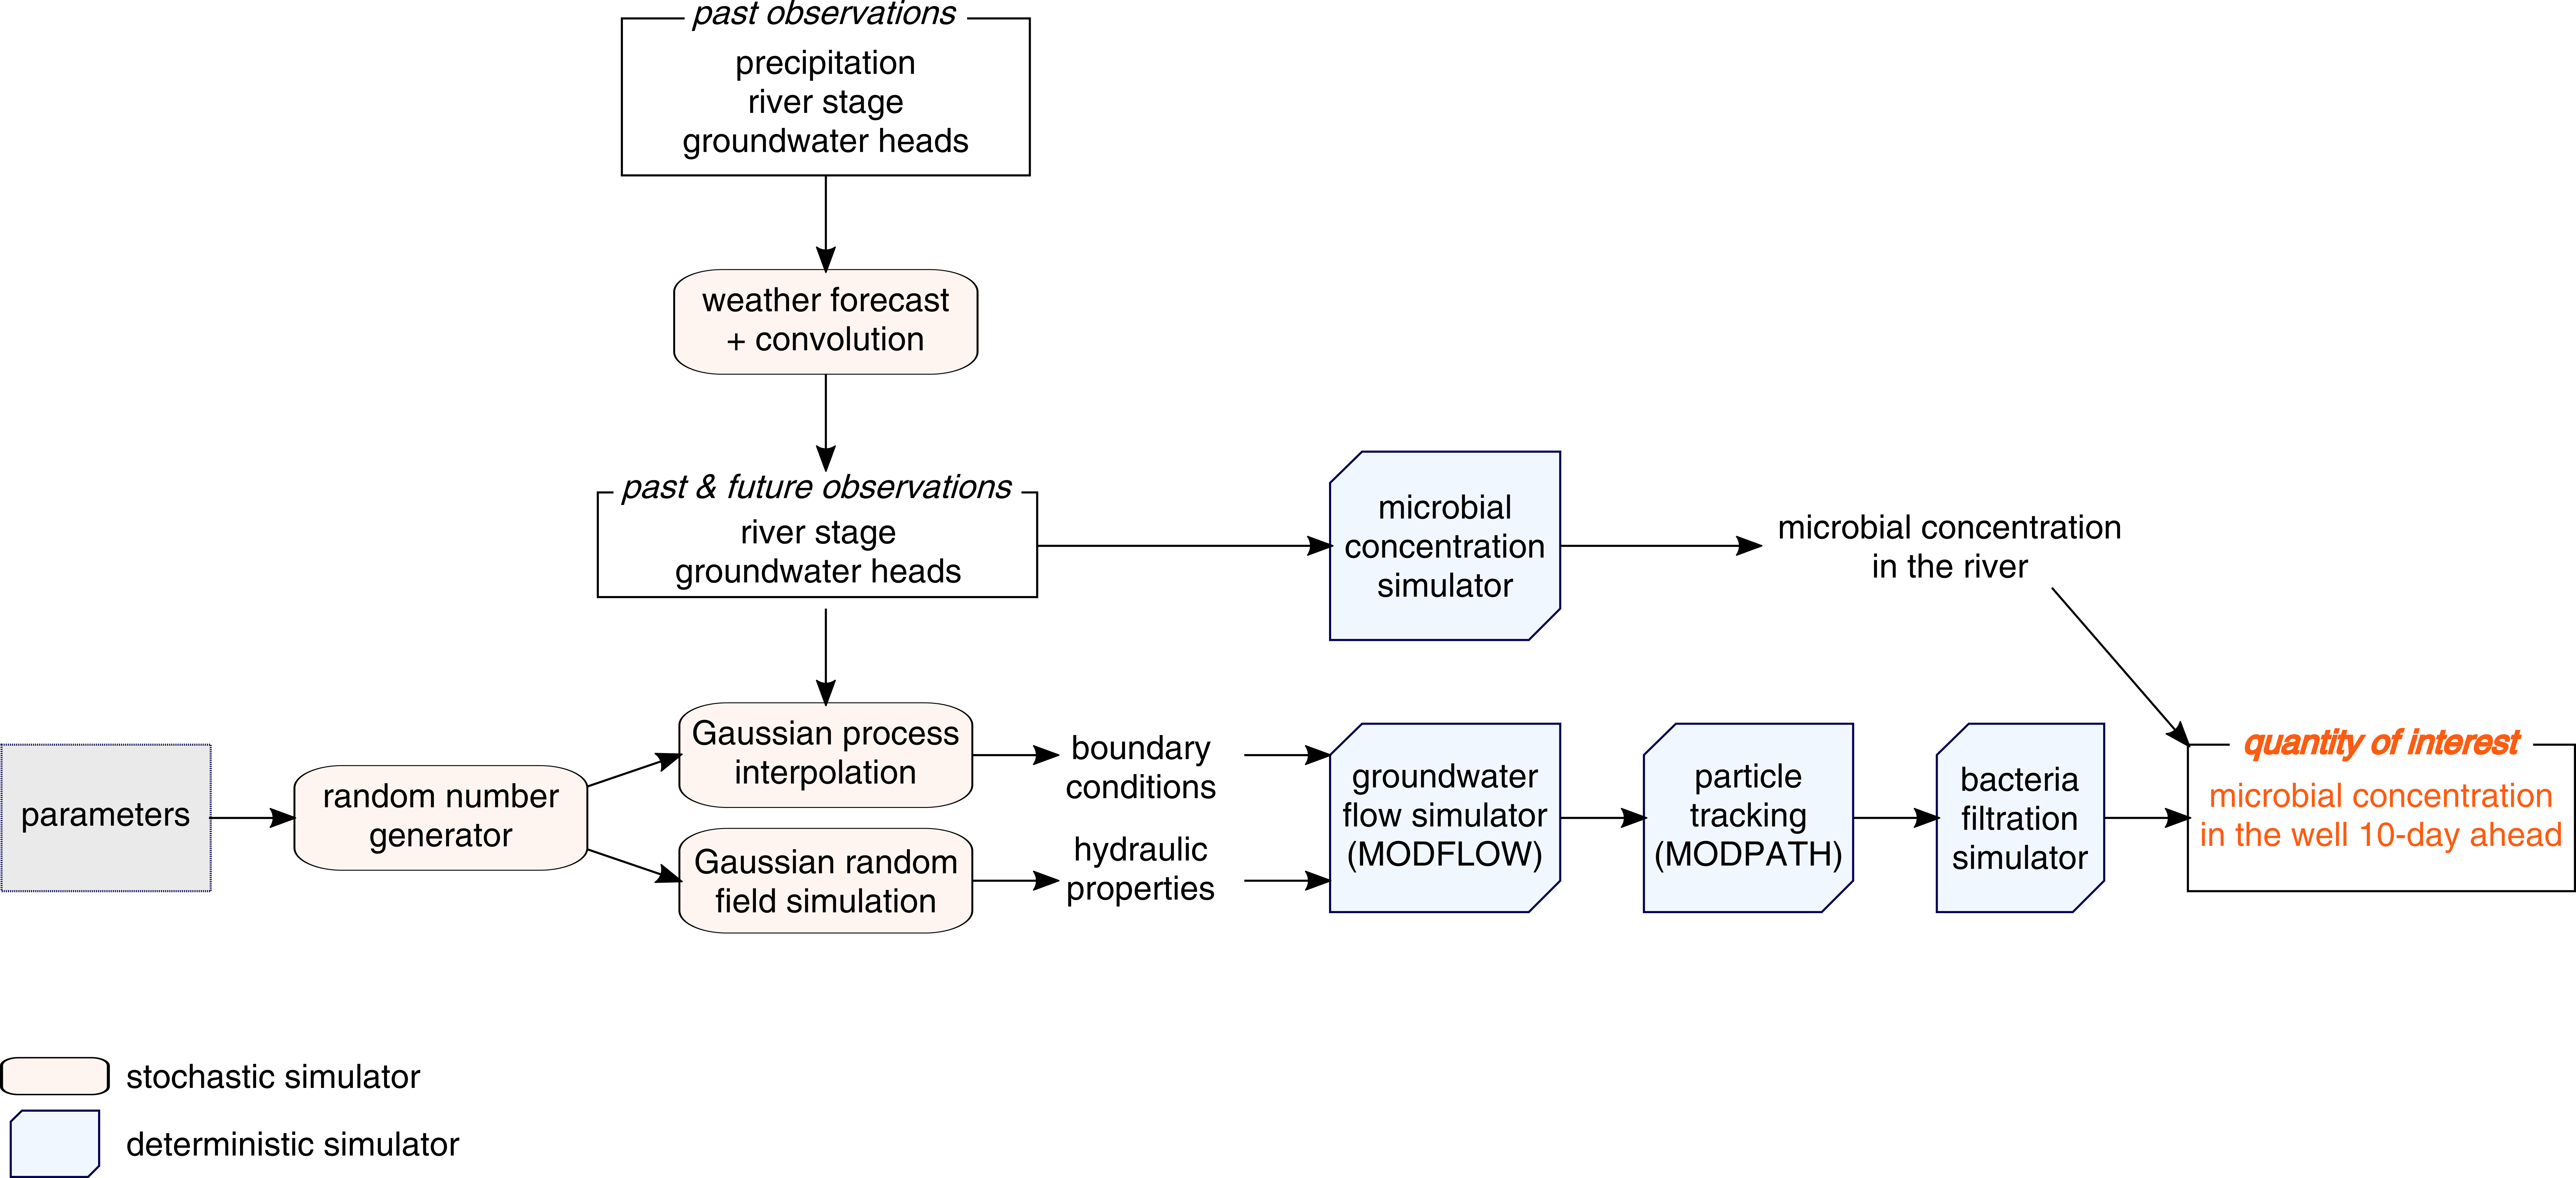
\includegraphics{imgPres/gwModBac_model_overview.png}

\end{block}

\end{frame}

\begin{frame}{Modflow -stochastic simulation (2)}

\columnsbegin

\column{.4\textwidth}

Bacteria pathways

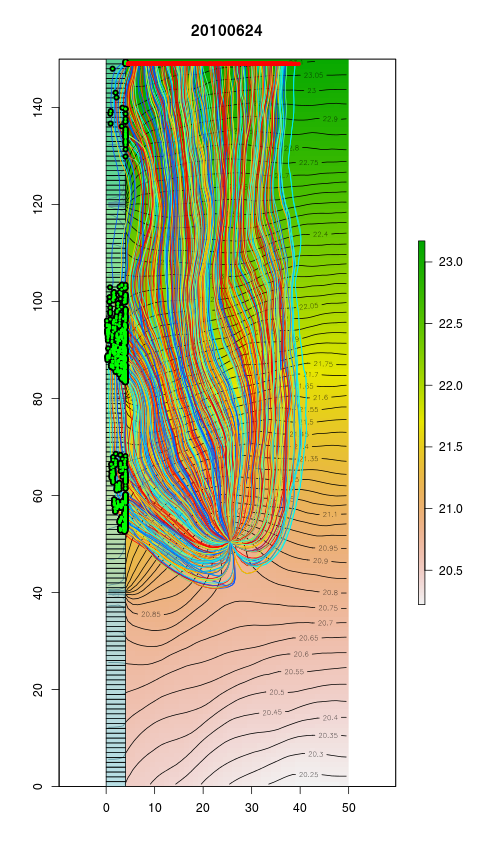
\includegraphics{imgPres/gwModBac_rea_0001.png}

\column{.6\textwidth}

Bacteria concentration as a function of grid size

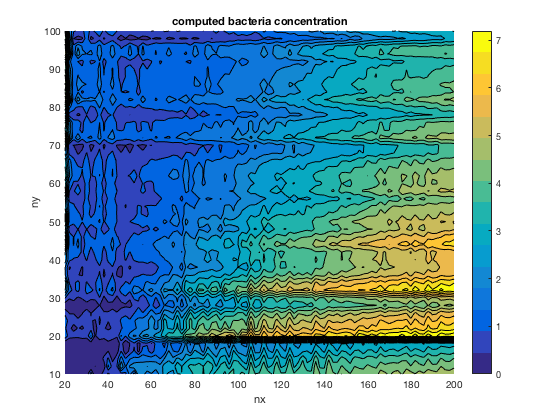
\includegraphics{imgPres/gwModBac_concentration_2.png}

\columnsend

\end{frame}

\begin{frame}{physically based lumped model}

simulate groundwater fluctuations in response to precipitation and
pumping: \href{https://cran.r-project.org/package=ambhasGW}{package
ambhasGW} \href{www.mdpi.com/2071-1050/10/1/26/pdf}{Sekhar et al.
(2017)}

\end{frame}

\section{Reporting}\label{reporting}

\begin{frame}[fragile]{publication-quality figures (see also package
\texttt{ggplot2})}

Either:

\begin{itemize}
\item
  \texttt{ggplot} and \texttt{ggplot2} and theirs cousins
\item
  or base \texttt{graphics}, \texttt{plot3D}
\item
  3D interactive plot with \texttt{rgl} (based on OpenGL)

\begin{Shaded}
\begin{Highlighting}[]
\KeywordTok{library}\NormalTok{(rgl)}
\KeywordTok{demo}\NormalTok{(abundance) }
\end{Highlighting}
\end{Shaded}

  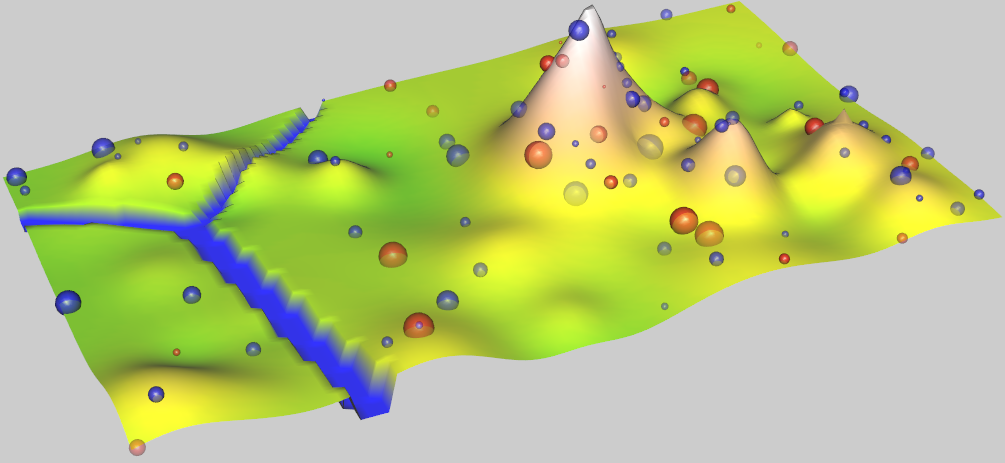
\includegraphics[width=0.60000\textwidth]{imgPres/rgl_demo.png}
\item
  Report/presentation/book: HTML/PDF (packages \texttt{RMarkdown} and
  \texttt{knitr})
\item
  interactive web apps (package \texttt{shiny})
\item
  R package (code and/or data)
\item
  R can create interactive teaching modules: You can do it in the
  console with \texttt{swirl} or on the web with \texttt{Datamind}.
\end{itemize}

\end{frame}

\section{Check}\label{check}

\begin{frame}{check}

\begin{quote}
In short, pair-wise x-y plots were computed between the average
baselines of all FCM and sensor parameters for a first visual
observation of any apparent correlations. The pair-wise correlations
between the full base- lines of all parameters were then quantified by
the computation of Pearson's correlation coefficients (PCC, linear
relationship) and Spearman's rank correlation coefficients (monotonic
rela- tionship) after standardization of the FCM and sensor data sets
(see Section 8 in supplementary information). The significance of the
correlations was assessed by the computation of p-values at 95\%
confidence level. The pair-wise coefficients were displayed in a heat
map for efficient representation of the gradients in pos- itive and
inverse correlations between parameters, and for rapid identification of
the pre-dominant correlations. In this heat map, the parameters were
reordered by hierarchical clustering using the Ward algorithm (see
Section 8 in supplementary information). The additional R packages Vegan
(Oksanen et al., 2009), Heatplus (Ploner, 2011), and Heatmap.plus (Day,
2007) were used to these ends.
\href{https://www.baselland.ch/politik-und-behorden/direktionen/bau-und-umweltschutzdirektion/umweltschutz-energie/wasser/wasserversorgung/publikationen/downloads/tp1-karstsysteme.pdf}{TP1
Basellandschaft}
\end{quote}

\begin{quote}
Online flow cytometry measurements were linearly interpolated and then
sampled at equal time intervals (15-minutes) using the ``approx()''
command of the statistical software R39. This was to adjust for minor
deviations from the 15-minutes sampling interval in the original data
set\ldots{}
\end{quote}

\begin{quote}
\ldots{}The interpolated time series was then decomposed into a ``trend
component'' (aperiodic dynamic), a ``seasonality component'' (periodic
dynamic; R-code based terminology not related to seasons of the year),
and a ``remainder component'' (noise and dynamics not accounted for by
the above two components) using the ``stl()'' command\ldots{}
\end{quote}

\href{https://www.nature.com/articles/srep38462}{Nature}

\begin{quote}
Understand what you are doing!
\end{quote}

check
\href{http://uribo.github.io/rpkg_showcase/date_and_time/zoo.html}{check}

\end{frame}

\section{Great tool for coding, reporting and code
maintaining}\label{great-tool-for-coding-reporting-and-code-maintaining}

\begin{frame}{RStudio}

\begin{itemize}
\tightlist
\item
  package creation and development
\item
  reporting with Rmarkdown
\end{itemize}

\end{frame}

\begin{frame}{
\includegraphics[height=0.33333in]{imgPres/input/git-logo.png}
\& 
\includegraphics[height=0.33333in]{imgPres/input/github-logo.png}}

git = a free and open source distributed version control system

github = a web-based hosting service for version control using git

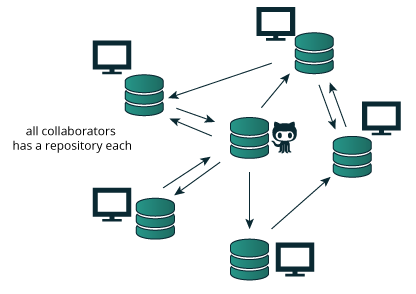
\includegraphics[width=0.60000\textwidth]{imgPres/input/distributed-vc.png}

\begin{quote}
Open source means everyone can see my stupid mistakes (Karl Broman)
\end{quote}

\begin{quote}
Version control means everyone can see every stupid mistake I've ever
made (Karl Broman)
\end{quote}

\end{frame}

\begin{frame}{Reproducible research (1)}

\begin{quote}
Karl -- this is very interesting , however you used an old version of
the data (n=143 rather than n=226).

I'm really sorry you did all that work on the incomplete dataset.

Bruce
\end{quote}

from Karl Broman

\end{frame}

\begin{frame}{Reproducible research (2)}

from Karl Broman

\begin{enumerate}
\def\labelenumi{\arabic{enumi}.}
\setcounter{enumi}{-1}
\tightlist
\item
  Separate the raw data from everything (and don't modify them)
\item
  Organize your data \& code
\item
  Everything with a script
\item
  Automate the process (GNU Make)
\item
  Turn scripts into reproducible reports
\item
  Turn repeated code into functions
\item
  Create a package/module
\item
  Use version control (git/GitHub), no more
  ``really\_true\_final\_2EH5b.doc''
\item
  Pick a license, any license
\end{enumerate}

\end{frame}

\end{document}
